% Template for Biophysics paper in LaTeX
%
% To compile into a document, run
% latex biophys_latex_template
% bibtex biophys_latex_template (if bib file and bst file is included in TeX file)
% latex biophys_latex_template (run 2-3 times repeatedly)
% dvips biophys_latex_template.dvi
%
% or replace the latex command by the pdflatex command in the lines above to
% generate a PDF file and use acroread or xpdf for viewing and
% printing instead of the postscript generating program dvips

% Use standard biophys document class with default font size
% and typeset in one column. If you need to typeset in two column
% then give the option "twocolumn" ie \documentclass[twocolumn]{biophys}
\documentclass[twocolumn]{biophys}
\usepackage{helvet,times}
\usepackage{bm,textcomp}

\jno{kxl015} %journal number
\gridframe{N}%option for grid around the text "Y" or "N"
\cropmark{N}%option for cropmark around the text "Y" or "N"

\doi{doi:15}% DOI number in the copyright line

%The first page number and last page number automatically generated.
%To change the page number \setcounter{page}{10} automatically reset
%the first and last page number but two times compilation required.
%If you want to edit the page range in catch line
% then edit the below two lines
%\fpage{}
%\lpage{}
%For update volume number, activate below command
%\volume{00}
%For update issue number, activate below command
%\issue{00}
%For update Month, activate below command
%\Month{Month}
%For update Year, activate below command
%\Year{Year}


% Packages to load (all standard on a modern LaTeX system on Linux)

% Make doublespaced ugly typography required for mysterious
% reasons by most journals - comment out for normal output
%\usepackage{setspace}
%\doublespacing
% AMS-Math package to have nice multi-line equations and other goodies
\usepackage{amsmath}
% Show labels for easy orientation, comment out for final version
% \usepackage{showlabels}

% EPS/PDF graphics
% Place figures in the document directory in both the EPS and PDF
% formats, e.g., fig_1.eps and fig_1.pdf. Use the includegraphics
% command without file extension, e.g. \includegraphics*[width=3.25in]{fig_1}
% The pdflatex or latex programs then work automagically with the
% appropriate formats.  EPS figures can be converted to PDF using
% the epstopdf program present on most Linux disributions. Epstopdf and graphicx
% are included in biophys class file.
% \usepackage{graphicx}

% Citation style in the text: numbers in parenthesis, sorted by their
% order in the list of references.
% Uses a range if possible: (1-3), not (1,2,3)

\usepackage{algorithm}
\usepackage[noend]{algpseudocode}
\usepackage{caption}
\usepackage{subcaption}
\usepackage{graphicx}
\usepackage{textcomp}
\usepackage{amsfonts}
\usepackage{dsfont}
\usepackage{gensymb}
\usepackage{caption}
\usepackage{epstopdf}
\usepackage{mathtools}

\usepackage[round,numbers,sort&compress]{natbib}

% Bibliography style (requires the style file biophysj.bst in the
% document directory)

%\bibliographystyle{biophysj}

% Numbering style in the list of references: a number followed by a period

\renewcommand{\bibnumfmt}[1]{#1.}

\epstopdfsetup{outdir=./}
\graphicspath{{../}}
% Examples of special definitions (amsmath package required)
\newcommand{\erf}{\operatorname{erf}}        % error function
\newcommand{\erfc}{\operatorname{erfc}}      % complementary error function
\newcommand{\BibTeX}{\textsc{Bib}\TeX}       % corect BibTeX appearance
\DeclarePairedDelimiter\floor{\lfloor}{\rfloor}
\makeatletter
\def\BState{\State\hskip-\ALG@thistlm}
\def\mean#1{\left< #1 \right>}
\makeatother


% Running head


\markboth{Biophysical Journal: Biophysical Letters}{Biophysical Journal: Biophysical Letters} %for running head

% We are done with the headers, the actual document starts here




\begin{document}



\setcounter{page}{1} %first page number

\title{Using mathematical modelling to explore mRNA localization}

\author{Jonathan Harrison \authdagger, Richard Parton \textsuperscript{$\ddagger$}, Ilan Davis \textsuperscript{$\ddagger$}, Ruth Baker \authdagger}

\address{\addrdagger Mathematical Institute, University of Oxford; \textsuperscript{$\ddagger$} Department of Biochemistry, University of Oxford}


% generate the title page from the info in the headers above


%Abstract environment needs 3 arguments. They are
%1. The abstract
%2. Received date
%3. Address, email

\begin{abstract}%
{In early \textit{Drosophila} development, mRNA localization plays a key role in determination of the body axes. 
Maternal mRNA is transported from the nurse cells into the oocyte itself, where it is localized to specific sites in order to target proteins to regions where they can function. 
We investigate the rate-limiting steps of mRNA localization and targets for regulation by the cell.
By employing a simple velocity jump process model of the transport of mRNA, we describe this transport process and demonstrate how it depends on certain parameters of the model, such as the bias in the microtubule network.
The model used represents the active transport and diffusion phases observed experimentally.
Based on simulations from the model with inferred parameters, we estimate a mean first passage time from the nucleus of the nurse cell to the ring canal joining to the oocyte of 18 min. 
Since the timescales over which mRNA localization occurs during oogenesis are at least an order of magnitude longer than this, we suggest that production is the rate-limiting step in mRNA localization. 
Finally, we incorporate production of mRNA complexes directly into our model and are thus able to reproduce a spatial distribution of mRNA complexes similar to experimental observations.
Mathematical modelling can offer mechanistic insight into this system by providing testable hypotheses and informing experimental design.
%In future, this modelling approach could be applied to improve tracking of individual mRNA complexes. 
}%1
{}
{}
\end{abstract}

\maketitle %%The above information typeset through this command

\section{Introduction}

The localization of mRNA is crucial in a variety of biological contexts for the targeting of proteins to their site of function.
%This enables proteins to be
This method of gene expression is particularly relevant for polarized cells such as oocytes and early embryos.
For example, the axes of \textit{Drosophila Melongaster} are established through regulation of gradients in \textit{bicoid} (\textit{bcd}), \textit{gurken} (\textit{grk}), \textit{oskar} (\textit{osk}) and \textit{nanos} (\textit{nos}) mRNA \citep{wolpert1998}.
mRNA localization has been observed in a variety of species and cell types, including \textit{Drosophila} and \textit{Xenopus} oocytes, neurons, chicken fibroblasts, yeast and bacteria \citep{wilkie2001drosophila, bobola1996asymmetric, mowry1992vegetal, rosbash1993rna, nevo2011translation}, thus demonstrating that this process is ubiquitous and not limited to large cells. 
\textit{Drosophila} relies heavily on the asymmetric locatization of mRNAs to coordinate early development processes both spatially and temporally.
This makes Drosophila an ideal model system for the study of mRNA localization.

Recent advances in imaging techniques and image analysis technologies \citep{jeffery1983localization, bertrand1998localization, hamilton2010particlestats} have advanced our understanding of the mechanisms of mRNA localization. 
The use of flourescence \textit{in situ} hybridisation (FISH) enables single molecules of mRNA to be labelled with high levels of sensitivity and specificity. 
The development of the MS2-MCP system, which consists of a MS2 bacteriophage RNA stem loop bound by MS2 coat protein fusion to a flourescent protein \citep{parton2014subcellular}, has provided great benefits for the imaging of live cells \textit{in vivo}.
The MS2-MCP system has been used successfully in the visualisation of \textit{nos}, \textit{grk}, \textit{bcd} and \textit{osk} mRNAs in Drosophila \citep{forrest2003live, jaramillo2008dynamics, weil2006localization, zimyanin2008vivo}.
Although there are limitations to these technologies dependent on cell type, they have permitted an improvement of our understanding of intracellular motility.
What has become clear is that a variety of different mechanisms are used to ensure localization of mRNAs.

What is not yet well understood are the molecular mechanisms used in the mRNA localization process and why such a variety of transport methods are present.
It is likely that this aids regulation and the movement of different mRNAs in parallel.

\subsection{Motivation}
After transcription and transport out of the nucleus, many mRNAs are localized and translated in the distinct cytoplasmic domains where they function \citep{jansen2001mrna, parton2014subcellular}.
This process is highly regulated and involves active transport by intricate molecular motors.
mRNA localization is crucial for the establishment of polarity of cells and the formation of the basic animal body plan during development \citep{wolpert1998}. 
It may have importance for a wide range of functions involving memory and learning in the nervous system. 
However, we are a long way from a complete understanding of the mechanisms governing the mRNA cargo transport process.

In particular, the mRNA transcripts that set up the \textit{Drosophila} body axes originate in the nurse cells (see Figure \ref{FIG:Drosophila_development}) and are actively transported on microtubules into the oocyte through the ring canals \citep{clark2007dynein}.
We will focus on this maternal transfer of transcripts into the oocyte, since this area has been less well studied and it is tractable both to modelling and data collection.
\begin{figure}[h]
 \centering
 \includegraphics[width=\columnwidth]{/home/harrison/Documents/mRNA/Figures_for_writeup/Drosophila_development_grk_labelled.png}
 \caption{\small Stages of \textit{Drosophila} development, showing nurse cells labelled as nc, follicle cells denoted by fc and the oocyte marked as oo. The localization of \textit{grk} is shown in blue. Adapted from \citet{lasko1999rna}.}
 \label{FIG:Drosophila_development}
\end{figure}

One of the challenges involved in live imaging of cells to examine this transport process is the need to scan a sample in three spatial dimensions as well as in time.
This places restrictions on the resolution of the data that can be obtained temporally and in the $z$ direction due to the limitations of current imaging technologies \citep{weil2010making}.
Although there are physical restrictions on what can be achieved by improvements in imaging technologies, these could be overcome by modelling of the transport of mRNA cargoes, which may permit sparser sampling in time and finer sampling in space.
By simulating from our model, assuming we have knowledge of the current state of a particle and appropriate values for model parameters, we can predict a likelihood for the state of a particle after a short time $\Delta t$.
This could be used to inform the linkage step to identify particles between frames and may allow larger timesteps $\Delta t$ to be taken between imaging frames, although a hidden Markov model (HMM) framework may be necessary to update the current state of the particle.
An HMM approach has previously been applied to tracking in the context of bacteria \citep{rosser2013novel} and for single-molecule diffusive protein data \citep{persson2013extracting}.

Through mathematical modelling of mRNA transport in the \textit{Drosophila} nurse cell, we aim to better understand the limiting factors in mRNA localization.
This will improve our understanding of which parts of the process are important biologically for its function and should give insight into the molecular mechanisms used by informing future experimental design.
In addition, we see the potential for this modelling framework to be applied using an HMM framework to improve tracking of RNP complexes over longer time periods in three-dimensional data.

\subsection{Outline of mRNA localization process} \label{Outline}

Once mRNA has been transcribed from DNA in the nucleus, the process by which it reaches its final site of localization, where it is then translated into protein, can be divided into four main stages: particle formation; nuclear export; transport; and anchoring.
We will address each of these processes in turn.
Understanding of these stages will enable the development of our model in Section \ref{Modelling}.

mRNA does not exist in isolation inside the cell.
Instead the mRNA molecules bind to proteins to form particle complexes, which are also known as ribonuclearproteins (RNPs). 
These proteins perform a range of different functions, including translational regulation, preventing translation while the mRNA is in transit, and may determine the final destination of the particle \citep{hamilton2013multidisciplinary}.
%Examples of proteins that form these particles include \textit{Squid} (\textit{sqd}) and \textit{Orb}.
There is also evidence that RNPs are dynamically remodelled during the transport process, to support translational regulation \citep{weil2012drosophila}.

After the mRNA has assembled into RNPs, it must diffuse through the crowded interchromatin spaces in the nucleus until it reaches a nuclear pore complex (NPC).
The RNP is then exported out of the NPC into the cytoplasm via interactions with co-factors.
Certain NPCs are more active than others at different times \citep{weil2012drosophila}, but the overall direction of export out of the nucleus is unbiased \citep{wilkie2001drosophila}. 

The transport stage of mRNA localization occurs by different mechanisms for different mRNAs.
The most common method observed is transport via molecular motors moving along the cytoskeleton (either microtubules or actin filaments). 
However, \textit{nos} mRNA localizes using a diffusion and trapping technique \citep{forrest2003live} rather than by active transport. 
Active transport results in fast, directed motion with velocities of the order of $1 \mu \text{m} \text{s}^{-1}$ \citep{weil2006localization, zimyanin2008vivo, DavidsonPhD2015}, which is an order of magnitude faster than movement by free diffusion.
Bidirectionality was observed by \citet{vendra2007dynactin} in the Dynein mediated motion of RNP complexes on microtubules in \textit{Drosophila} blastoderm embryos.
It should be noted that, conventionally, individual types of molecular motors are thought to move unidirectionally, with Dynein directed towards the minus end of microtubules and Kinesin directed towards the plus end \citep{howard2001mechanics}.
The number of motors required for a given RNP complex can vary and may be governed by cis-acting localization elements in the mRNA \citep{amrute2012single}.
Possible explanations for the bidirectionality include: a tug of war between different molecular motors moving in opposing directions on different microtubules; a tug of war between different motor species all bound to the same RNP complex; reversal of Dynein moving on a single microtubule, possibly due to regulation by microtubule associated proteins (MAPs) \citep{buxbaum2015right}. 
The molecular motors must be correctly joined to their cargo and the motor cargo complex secured to the cytoskeleton.
This is ensured in \textit{Drosophila} oocytes by the linkers \textit{Bicaudal D} (\textit{BicD}) and \textit{Egalitarian} (\textit{Egl}) \citep{parton2014subcellular}. 
The cytoskeleton was initially thought to be a stable static network, due to how it was analysed in fixed material.
However, it has recently been revealed, in \textit{Drosophila} oocytes, to be a dynamic network with a biased random orientation of microtubules \citep{parton20111}.
This underlying structure had been suggested by the work of \citet{zimyanin2008vivo} who observed RNPs containing \textit{osk} mRNA moving in a biased random walk.  

Once the RNP complex has reached its destination, it must be maintained in position to keep the mRNA localized within the cell.
In many cases an anchoring mechanism is used; \textit{grk} mRNA is anchored by the molecular motor Dynein \citep{delanoue2005dynein} in the \textit{Drosophila} oocyte and \textit{nos} is trapped by actin \citep{forrest2003live}.
Dynein was observed by \citet{delanoue2005dynein} to act as a static motor without requiring further energy in the form of ATP to function. 
An alternative hypothesis is that continuous active transport is required to ensure the localization of mRNA, since \citet{weil2006localization} found that Dynein motor activity is required to ensure \textit{bcd} localization in the anterior cortex of the Drosophila embryo.
The transport process may ensure that RNP complexes are kept near their targeted region of localization by directing them back if they move away.

In this work, we present a simple model for transport of mRNA particles through nurse cells during localization and demonstrate how this model can be effectively parametrised.
In Section \ref{Methods}, we construct the velocity jump process model and explain the approximate Bayesian computation (ABC) approach to inference of the model parameters.
We exhibit the posteriors over the model parameters generated via our inference approach for both \textit{in silico} and \textit{in vivo} data in Section \ref{Results}.
Finally, in Section \ref{Conclusions}, we discuss some of the implications of our modelling and parameter inference, before exploring possible future directions.

\section{Materials and Methods} \label{Methods}
\subsection{Modelling approach} \label{Modelling}
In this context, modelling involves breaking down the mRNA localization process into its key components and identifying the biologically important aspects. 
We put in place appropriate, simple modelling assumptions to describe the most important parts of the system biologically.
These assumptions should as far as possible be supported by existing experimental observations, as described in Section \ref{Outline}.

Previous modelling approaches in this area have focused on descriptions of the mechanisms driving molecular motors at smaller spatial and temporal scales \citep{bressloff2013stochastic} or with continuous densities of mRNA \citep{szymanska2014mathematical} rather than representing single RNP particles which would be more appropriate at low densities.
Other studies have generally considered mRNA dynamics in the oocyte in terms of cytoplasmic streaming or diffusion without direct reference to active transport \citep{ganguly2012cytoplasmic, liu2011role}.
Instead we shall describe the active transport of mRNA in the nurse cells surrounding the ooctye, which are connected to each other and to the oocyte via ring canals, using an individual-based stochastic description.

We propose two different approaches to parameterize our model. 
The first will involve direct measurement of parameters, such as the average speed of cargo complexes during periods of active transport.
The second method requires application of an ABC framework \citep{johnston2014interpreting, turner2012tutorial, beaumont2002approximate} to parameterize the model via comparison with certain summary statistics of the data.
This will enable comparison between the experimentally measured parameter values and the posterior for these parameters obtained via ABC.

We aim to produce a testable model in the sense that we are able to make predictions from the model based on varying certain parameters, such as the speed of the motor carrying the cargo. These could be tested experimentally using genetic mutants that have behaviour that corresponds to a different value of a given parameter. 
This should inform our understanding of how transcripts transport and localize.

\subsection{Velocity jump process} \label{VJ model}
The movement of RNP cargoes is often described as a biased random walk \citep{zimyanin2008vivo}.
Rather than modelling this transport process as a simple random walk in position, we let the direction of motion vary. 
This type of model is known as a velocity jump process and has been successfully applied to directed migration of animals and cells \citep{codling2005calculating, taylorking2015birds}.

\begin{figure}[h]
 \centering
 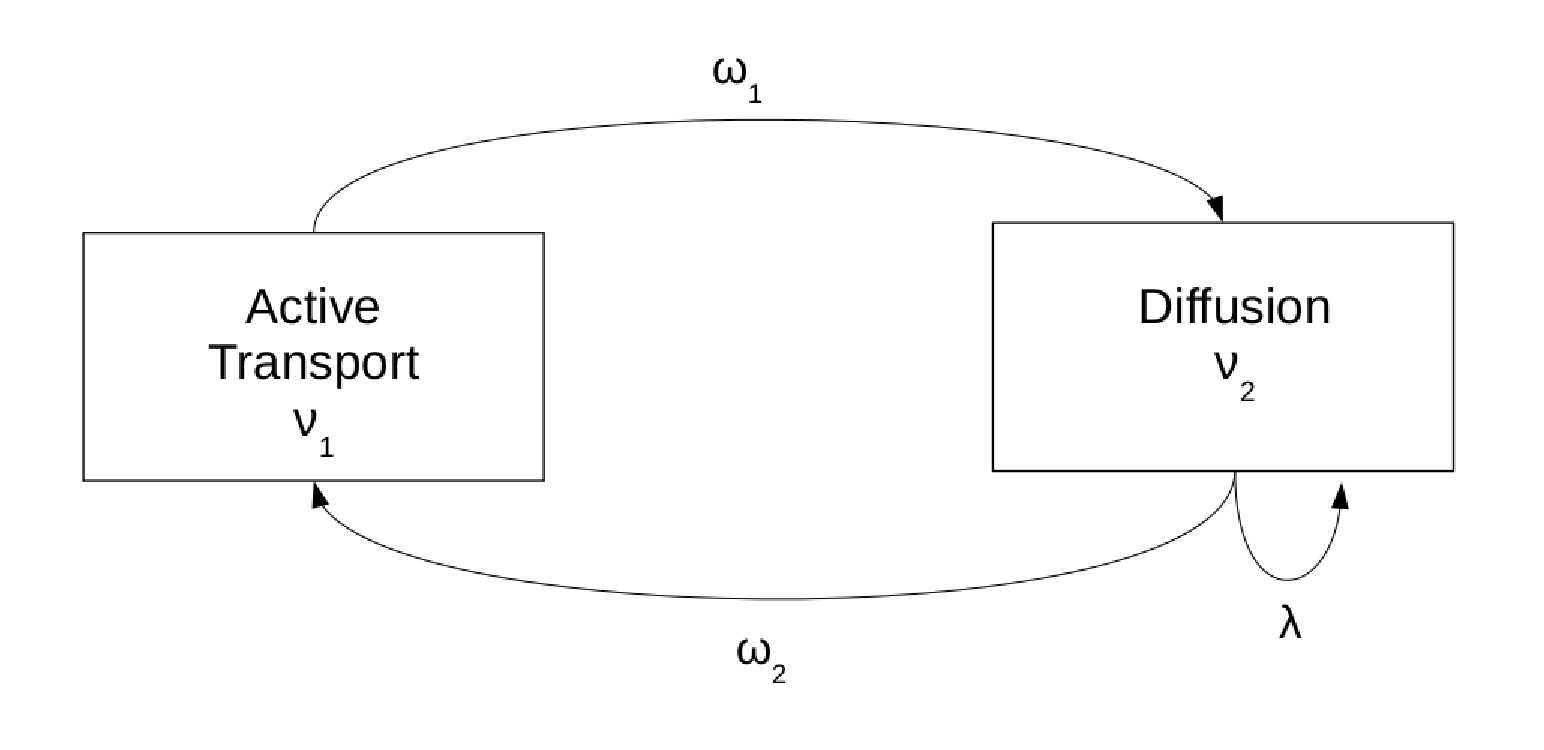
\includegraphics[width=\columnwidth]{/home/harrison/Documents/mRNA/Figures_for_writeup/States_diagram.eps}
 \caption{\small States and transitions between the states in the velocity jump process model. The speeds in active transport and diffusion are $\nu_1$ and $\nu_2$, respectively. Transition rates between states are given by $\omega_1$, $\omega_2$ and $\lambda$, as shown.}
 \label{FIG:Phases_of_motion}
\end{figure}

We model a two-dimensional slice through a nurse cell as a rectangular region $[0,L_x] \times [-L_y/2, L_y/2]$, with the $x$ axis aligned along the anterior-posterior axis of the oocyte.
The cell nucleus is modelled as a circular region of given radius, $R$, placed centrally in the cell. 
This is excluding to the RNP complexes in the model which are reflected by it.
The remainder of the nurse cell is accessible to the particles, which seems reasonable since experimentally particles are observed in all parts of the nurse cell (data not shown).
Initially, RNP cargoes are placed randomly at time $t=0$ on the circumference of the nucleus to represent their export from nuclear pore complexes.
In the model therefore, all mRNAs are produced simultaneously rather than directly modelling continual production and export over time.
Cargoes move randomly, as described below, until eventually they hit a small target at the posterior end of nurse cell representing the ring canal joining to the oocyte, where they are absorbed and removed from the system.
Throughout all simulations in this work, we fix $L_x=52 \mu \text{m}$, $L_y=37 \mu \text{m}$, $R=10 \mu \text{m}$ and the size of the ring canal as $2\mu \text{m}$, based on measurements taken of nurse cells in earlystages of oogenesis.
The position of the ring canals between the nurse cells and the ooctye can be clearly seen in Figure \ref{FIG:ring_canals}.
The geometry of the model system can be seen in Figure \ref{FIG:geometry} and contrasted with a real nurse cell.
\begin{figure}[h]
 \centering
 \includegraphics[width=\columnwidth]{/home/harrison/Documents/mRNA/Figures_for_writeup/Ring_canals_snap_01.jpg}
 \caption{\small Position of the ring canals between the nurse cells and the oocyte for a stage 5 \textit{Drosophila} oocyte. The ring canals are highlighted with Sqh Utrophin GFP and the red channel was obtained via differential inteference contrast microscopy.}
 \label{FIG:ring_canals}
\end{figure}

\begin{figure}[h]
 \centering
 \begin{subfigure}[b]{0.375\textwidth}
 \includegraphics[width=\columnwidth]{/home/harrison/Documents/mRNA/Figures_for_writeup/Ring_canals_snap_02.jpg}
    \caption[]%
  {{\small \textit{In vivo}.}}    
  \label{fig:vivo}
\end{subfigure}
 ~
  \begin{subfigure}[b]{0.475\textwidth}  
      \centering 
      \includegraphics[width=\textwidth]{/home/harrison/Documents/mRNA/Figures_for_writeup/Domain_geometry.eps}
      \caption[]%
      {{\small Model nurse cell domain.}}    
      \label{fig:model}
  \end{subfigure}
  \caption{\small Comparison of the geometrical structure of our model nurse cell and a nurse cell \textit{in vivo}. 
  In (\subref{fig:vivo}), Sqh Utrophin GFP was used to show the position of the ring canals in an oocyte in stage 8 of oogenesis. 
  In (\subref{fig:model}), the dashed black rectangular box shows the boundary of the nurse cell, with the solid black circle representing the nucleus, and the thick cyan line at the posterior showing the position of the ring canal between the nurse cell and the oocyte.}  
  \label{FIG:geometry}      
\end{figure}

There are two phases of motion included in the model: an active transport phase when the cargo is attached to the motor and is moving on the microtubules with constant speed $\nu_1$; and a slower diffusive phase with constant speed $\nu_2$.
Switching occurs between these two phases of motion with exponential waiting times between switching events.
Biologically this switching corresponds to the molecular motor falling off and reattaching to the microtubule.
As illustrated in Figure \ref{FIG:Phases_of_motion}, switching occurs from the active transport state to diffusion with rate $\omega_1$. 
From the diffusive phase, reorientations within the same phase occur with rate $\lambda$ and switching to the active transport phase takes place at rate $\omega_2$. 
At a reorientation event, the particle remains in the diffusive phase at speed $\nu_2$ and a new direction is picked uniformly on $[0,2\pi)$.
After each switching event from diffusion to the active transport state, the RNP complex also changes direction by picking a new direction of travel at random, where the angle $\theta $ is drawn from some distribution $T(\theta)$. 
Here we choose to define $T(\theta)$ empirically as uniform on $[0,\pi )$ and $[\pi, 2\pi )$ with a bias in favour of $[0,\pi )$ based on biological data.
We define a proportion of microtubules, $\phi$, aligned in the posterior direction (parallel to the $x$ direction in our model) and thus take the following for $T(\theta)$:
\begin{equation*}         
T(\theta) = \begin{cases} \frac{\phi}{\pi} &  \theta \in [0,\pi) \\ \frac{1-\phi}{\pi} &  \theta \in [\pi,2\pi).                       
\end{cases}
\end{equation*}

\subsection{Approximate Bayesian computation (ABC)}
In a statistical inference context, the likelihood of data given a certain set of parameters is a central quantity, particularly in calculation of the posterior over the parameters given certain data. 
The posterior is desirable as it offers more information than just point estimates of the model parameters.
Although for simple models it may be possible to evaluate the likelihood analytically, for more complex models the likelihood is often not tractable or is very expensive to compute.  
ABC techniques have been developed to address this issue \cite{beaumont2002approximate}.
Instead of directly evaluating the likelihood, ABC techniques assume it is possible to cheaply simulate from the model and use this to approximate the likelihood.

In an ABC rejection sampling approach we follow the procedure shown in Algorithm \ref{ABC-RS}, where $\pi(\theta)$ is a prior on the parameters, $\rho$ is a distance metric, $S(x)$ is a summary statistic used to summarize the data, $x$, and $\epsilon$ is a maximum tolerance for acceptance. 
%The accepted parameters $\theta$ then represent an approximation to the posterior distribution. 
\begin{algorithm}
\caption{ABC Rejection Sampling}\label{ABC-RS}
\begin{algorithmic}[1]
\State \textbf{for} $i=1$ \text{to} $n$  \{
\State Sample parameters $\theta$ from a prior on those parameters $\pi (\theta)$. 
\State Simulate data $x$ from the model $M(\theta)$ using those parameters. 
\State Calculate distance from observed data $y$: 
\If {$\rho (S(x),S(y)) < \epsilon $} accept the parameters $\theta$
\Else \hspace{2pt} reject the parameters $\theta$.
\EndIf
\State \}
\end{algorithmic}
\end{algorithm}

One drawback of this algorithm is that it depends on appropriate choice of the distance metric, $\rho$, the summary statistic, $S(x)$, and the tolerance, $\epsilon $. 
Clearly the quality of the posterior will depend on the choice of these hyperparameters, as, for example, increasing $\epsilon $ will decrease the quality of the corresponding posterior.
In some settings it may be possible to take the full data, rather than a summary statistic, and to set $\epsilon=0$ which would give an exact sample from the posterior, but in general this is not possible computationally. 
We can eliminate the importance of the tolerance to some extent by simulating $N$ samples from the prior, storing all the distances and keeping the closest $\alpha$ quantile of the sampled parameters to the observed data. 
The quality of the posterior still depends on $N$ and $\alpha$ but the choice of $\epsilon $, which may be dependent on other model parameters, is removed. 

The efficiency of the rejection sampling method is low, particularly for small values of $\epsilon$ as they entail tiny acceptance rates resulting in many wasted samples. 
More efficient ways of sampling possible parameters $\theta$ have been suggested including Sequential Monte Carlo and Population Monte Carlo techniques \citep{toni2009approximate, sisson2007sequential, beaumont2009adaptive, lenormand2013adaptive}.
%As such, we have opted to use an adaptive Population Monte Carlo (APMC) method  \citep{lenormand2013adaptive}. 

Inference on model parameters using ABC has been successfully applied to a variety of types of model in a biological context, often helping to offer biological insight into the model system.
Cell migration models have used ABC to process data from scratch assays \citep{johnston2014interpreting}, \textit{in vivo} data \citep{liepe2012calibrating}, and an individual-based ecological model with 14 parameters \citep{van2015calibration}. 

When using ABC methods, it is important to be aware also of their limitations. 
It has been highlighted via \citet{robert2011lack} that, although the error from the tolerance $\epsilon$ can be eliminated in the limit $\epsilon \rightarrow 0$, the use of summary statistics of the data may have larger effects, particularly when comparing models using ABC.
Some more systematic methods for choice of summary statistics have been suggested, which use minimization of certain measures of entropy to determine which summary statistics are most informative \citep{nunes2010optimal}.


\subsection{Imaging}
We observed \textit{grk}-MS2 mRNA in \textit{Drosophila} nurse cells tagged using MCP-Dendra and mcherry. 
Sqh Utrophin GFP was used to show the position of ring canals.
Imaging was performed with a wide-field deconvolution system (Delta Vision CORE) from Applied Precision. 
Image stacks were deconvolved with the SoftWoRx Resolve 3D constrained iterative deconvolution algorithm (Applied Precision). 
Segmentation of images was performed using Felzenszwalb's algorithm \citep{felzenszwalb2004efficient} after denoising and deconvolution of the images, with coordinates of particles obtained from centroids of appropriately sized segments. 
The age of egg-chambers was determined by measuring oocyte size and comparing known sizes at different stages of development.

\section{Results and Discussion} \label{Results}

\subsection{Direct parameter estimation}
Based on direct measurements from manually tracked grk-GFP mRNA complexes in \textit{Drosophila} nurse cells \citep{neuman1996drosophila}, we are able to make direct preliminary estimates of the parameters of our model.
All data were obtained from \citet{DavidsonPhD2015}.
Particles are classed as static, paused or active.
Paused and active particles will correspond to those in the diffusive and active transport phases of our model respectively. 
Static particles will be assumed to be either anchored or undergoing anomolous behaviour. 
The number of total particles counted was $N=340$ in a 40 $\times$ 40 $\mu \text{m}$ area.
The proportions of particles in each of the classes is $25\%$ active, $50\%$ paused and $21\%$ static. 
Over the timescale observed, particles did not transition between states and these are proportions of particles. 
Particle speeds were assessed by observing a 10 $\times$ 10 $\mu \text{m}$ area for 50 timepoints, with images taken in a single $z$ slice at three frames per second. 
The average speed in the active transport state $\nu_1 $ was  $1.163 \pm 0.08 \mu \text{ms}^{-1}$ from $n=33$. 
The average run length was $2.785 \pm 0.66 \mu \text{m}$. 
In the paused phase, an average speed, $\nu_2$, of $0.798 \pm 0.6 \mu \text{ms}^{-1}$ was observed from 58 particles with an average run length of  $0.84 \pm 0.06 \mu \text{m}$. 

Considering the process as a continuous time Markov chain, with active transport and diffusive states, we obtain that the steady state of the continuous time Markov chain is $[\omega_2 /(\omega_1 + \omega_2), \omega_1/(\omega_1+\omega_2)]$. 
Then assuming ergodicity and neglecting static particles, this approach gives us $\omega_2 /(\omega_1 + \omega_2) = 2/3$ and $\omega_1 /(\omega_1 + \omega_2) = 1/3$ by comparing to the proportions of particles observed in each state.
%Therefore the rates of falling off and reattaching must be different.

Assuming there are no internal transitions back to the active transport state, then we have $\omega_1 = 0.42 \text{s}^{-1}$ and hence $\omega_2 = 0.84 \text{s}^{-1}$. 
We can also deduce that the rate $\lambda = 0.95-0.84 = 0.11 \text{s}^{-1}$.  
In addition, we assume the distribution of microtubule orientations in the nurse cells is similar to that in the oocyte, since there is data available for the oocyte \citep{parton20111} but not for the nurse cell. 
Therefore we take $\phi = 0.58$.
This gives parameter estimates as shown in Table \ref{Table:Params}.
\begin{center}

 \begin{tabular}{| c | c |}
   \hline
   Parameter & Value \\ \hline
   $\nu_1$ & 1.16 $\mu \text{ms}^{-1}$ \\ %\hline
   $\nu_2$ & 0.8 $\mu \text{ms}^{-1}$ \\ %\hline
   $\omega_1$ & 0.42 $\text{s}^{-1}$ \\ %\hline
   $\omega_2$ & 0.84 $\text{s}^{-1}$ \\ %\hline
   $\lambda$ & 0.11 $\text{s}^{-1}$ \\ %\hline
   $\phi$ & 0.58 \\ %\hline
   $\gamma$ & 0.01 $\text{s}^{-1}$ \\
   \hline 
 \end{tabular}

 \end{center}
 \captionof{table}{Parameter values for the velocity jump process model.} \label{Table:Params}

\subsection{Timescales of the model}
Here, we evaluate the timescales of the transport phase of the localization process.
Based on simulations from the model, we obtain a mean first passage time (MFPT) from the nucleus to the posterior ring canal, averaged across 1000 particles, of $1070 \pm 840 \text{s} \approx 18 \text{min}$.
We plot the evolution of a typical path in Figure \ref{FIG:Typical_path}.
\begin{figure}[h]
 \centering
 \includegraphics[width=\columnwidth]{/home/harrison/Documents/mRNA/Figures_for_writeup/Typical_path.eps}
 \caption{\small The evolution of a typical path until absorption at the posterior ring canal. 
 Small black circles on the path show switching events between the active transport and diffusion states. 
 The geometry of the domain is as shown previously in Figure \ref{FIG:geometry}.}
 \label{FIG:Typical_path}
\end{figure}
Given that stage 5 in \textit{Drosophila} oocytes lasts five hours, this timescale for the MFPT appears to be an order of magnitude shorter than the timescales over which \textit{grk} mRNA transport is observed in oogenesis, suggesting that the limiting step in the transport and localization of the mRNAs is their production from the nucleus rather than the transport step.
We note that \textit{grk} mRNA complexes can be observed in the nurse cells from the germarium stage up until stage 8, when production of \textit{grk} appears to cease, as illustrated in Figure \ref{FIG:grk_localization}.
The distribution of particles visible in Figure \ref{FIG:grk_localization} also demonstrates that the difference in timescales is not due to a bottleneck elsewhere in the transport process, for instance at the ring canals, since no notable accumulation is seen there.
\begin{figure*}
 \centering
 \includegraphics[width=0.9\textwidth]{/home/harrison/Documents/mRNA/Figures_for_writeup/mcherry_stages.pdf}
 \caption{\small Localization of \textit{grk} mRNA at different stages of \textit{Drosophila} oogenesis. Increasing accumulation is seen in the oocyte over time. RNP particles can be seen in the nurse cell, until stage 8. The \textit{grk} mRNA was tagged with mcherry for visualization.}
 \label{FIG:grk_localization}
\end{figure*}

Furthermore, we are able to make predictions on what would happen if we halved the speed of the molecular motors via a genetic mutation.
We assume that altering the speed of the molecular motor, $\nu_1$, would leave the speed in diffusion, $\nu_2$, unchanged.
The resulting distribution is shown in Figure \ref{FIG:Half_speed_q} and the MFPT would be $2150\pm1600 \text{s} \approx 36\text{min}$.
\begin{figure}[h]
 \centering
 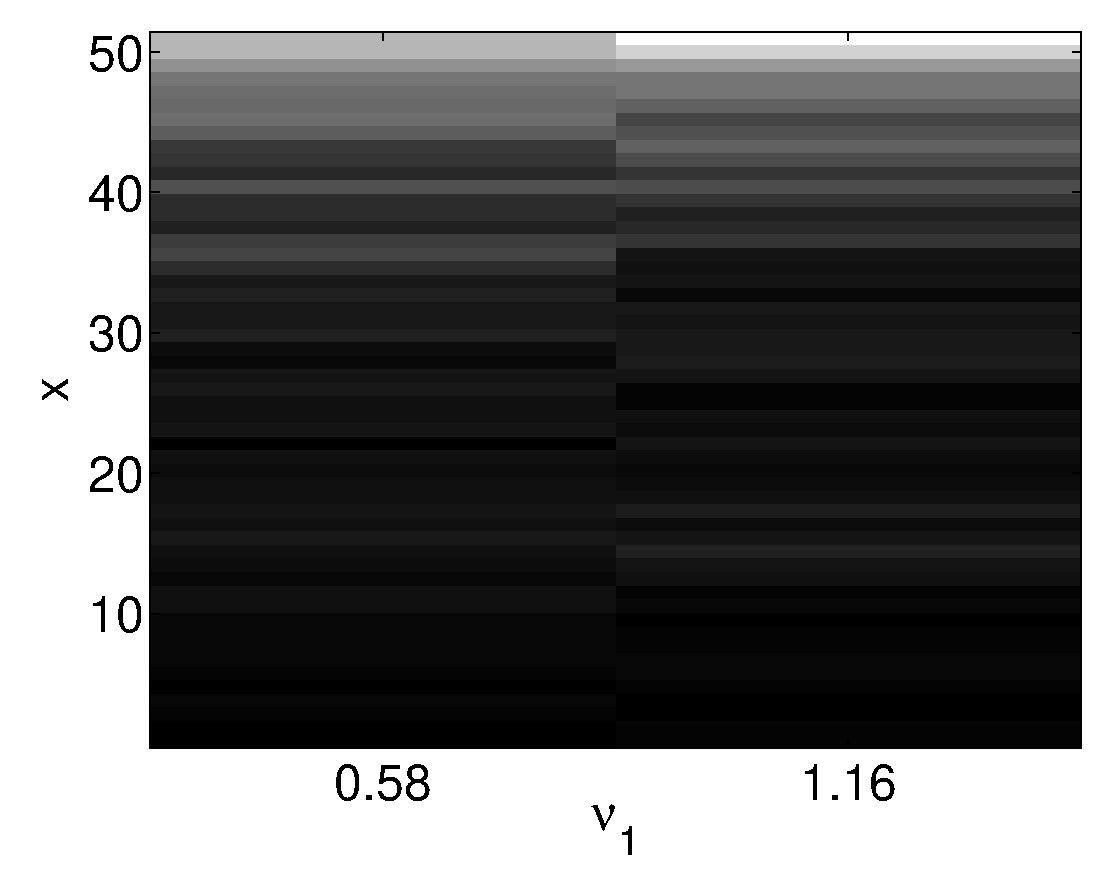
\includegraphics[width=0.85\columnwidth]{/home/harrison/Documents/mRNA/Figures_for_writeup/Spatial_distn_half_speed_mutant.eps}
 \caption{\small The spatial distribution resulting at time $t=270s$ from 1000 model simulations with parameters $\phi=0.58$, $\nu_2=0.8 \mu \text{ms}^{-1}$, $\omega_1=0.42 \text{s}^{-1}$, $\omega_2=0.84 \text{s}^{-1}$, $\lambda=0.11 \text{s}^{-1}$, varying $\nu_1$ as $0.58\mu \text{ms}^{-1}$ and $1.16\mu \text{ms}^{-1}$. 
 This represents the effect of introducing a genetic mutation to alter the speed of molecular motors.}
 \label{FIG:Half_speed_q}
\end{figure}

\subsection{Sensitivity analysis}
Our model is dependent on six parameters: $\nu_1, \nu_2, \omega_1, \omega_2, \lambda, \phi$. 
We are able to explore the dependence of our model on these parameters by performing a sensitivity analysis, varying each paramter over several orders of magnitude.
We show  in Figure \ref{FIG:Sensitivity_analysis} the effect of varying key parameters on the MFPT.
The results of this sensitivity analysis demonstrate that the turning rate within the diffusive state, $\lambda$, has no noticeable effect on this summary statistics (Panel \ref{fig:3lambda}).
Decreasing the speed parameters, $v_1$ and $v_2$, or the microtubule bias, $\phi$, leads to a sharp rise in the MFPT (Panels \ref{fig:3nu}, \ref{fig:3phi}). 
The transition rates $\omega_1$ and $\omega_2$ have opposite effects with an increase in $\omega_1$ increasing the MFPT, and a decrease in $\omega_2$ increasing the MFPT (Panels \ref{fig:3omega1}, \ref{fig:3omega2}). 
Similar effects are seen for two other summary statistics: the mean number of jumps on each path up to absorption, and the mean over different particles of the median jump distance on a single path, see Appendix \ref{Sensitivity_analysis_2}.

\begin{figure*}
        \centering
        \begin{subfigure}[b]{0.425\textwidth}
            \centering
            \includegraphics[width=\textwidth]{/home/harrison/Documents/mRNA/Figures_for_writeup/MFPT_phi.eps}
            \caption[]%
            {{\small Microtubule bias, $\phi$.}}    
            \label{fig:3phi}
        \end{subfigure}
        \hspace{1cm}
        \begin{subfigure}[b]{0.425\textwidth}  
            \centering 
            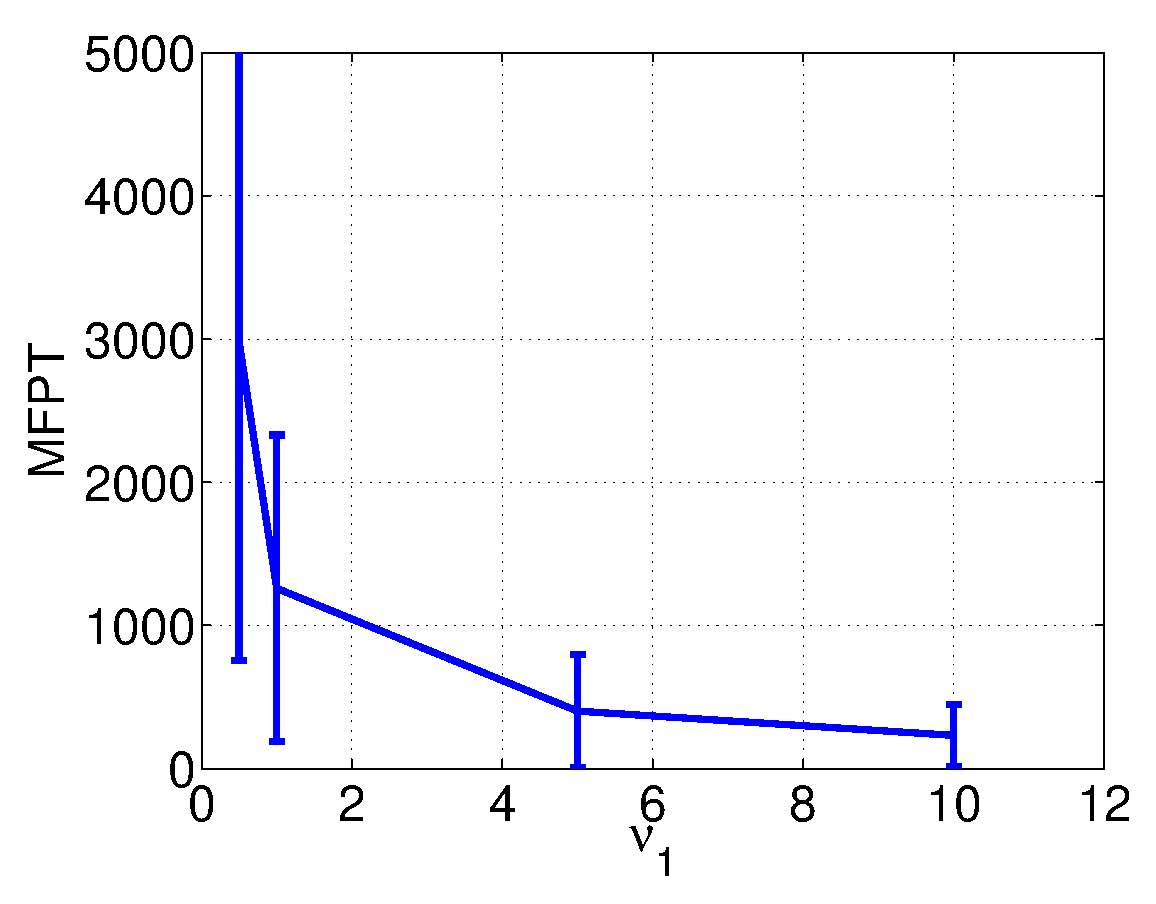
\includegraphics[width=\textwidth]{/home/harrison/Documents/mRNA/Figures_for_writeup/MFPT_nu.eps}
            \caption[]%
            {{\small Motor speeds, $\nu_1$ and $\nu_2$.}}    
            \label{fig:3nu}
        \end{subfigure}
        \vskip\baselineskip
        \hspace{3mm}
        \begin{subfigure}[b]{0.425\textwidth}   
            \centering 
            \includegraphics[width=\textwidth]{/home/harrison/Documents/mRNA/Figures_for_writeup/MFPT_omega1.eps}
            \caption[]%
            {{\small Switching rate to diffusion, $\omega_1$.}}    
            \label{fig:3omega1}
        \end{subfigure}
        \hspace{1cm}
        %\quad
        \begin{subfigure}[b]{0.425\textwidth}   
            \centering 
            \includegraphics[width=\textwidth]{/home/harrison/Documents/mRNA/Figures_for_writeup/MFPT_omega2.eps}
            \caption[]%
            {{\small Switching rate to active transport, $\omega_2$.}}    
            \label{fig:3omega2}
        \end{subfigure}
        \vskip\baselineskip
        \begin{subfigure}[b]{0.425\textwidth}   
            \centering 
            \includegraphics[width=\textwidth]{/home/harrison/Documents/mRNA/Figures_for_writeup/MFPT_lambda.eps}
            \caption[]%
            {{\small Reorientation rate in diffusion, $\lambda$.}}    
            \label{fig:3lambda}
        \end{subfigure}
        
        \caption{ \small Dependence of MFPT on the model parameters. Parameters used for simulations were $\phi=0.58$, $\nu_1=1.16 \mu \text{ms}^{-1}$, $\nu_2=0.8 \mu \text{ms}^{-1}$, $\omega_1=0.42 \text{s}^{-1}$, $\omega_2=0.84 \text{s}^{-1}$, $\lambda=0.11 \text{s}^{-1}$. For each of (\subref{fig:3phi}) to (\subref{fig:3lambda}), we vary a parameter in turn. 
        For (\subref{fig:3nu}), $\nu_2=\nu_1 / 2$ while varying $\nu_1$. Results are averaged over 100 particles with standard deviation shown on the error bars.}
        \label{FIG:Sensitivity_analysis}
    \end{figure*}

    
    \begin{figure*}
        \centering
        \begin{subfigure}[b]{0.425\textwidth}
            \centering
            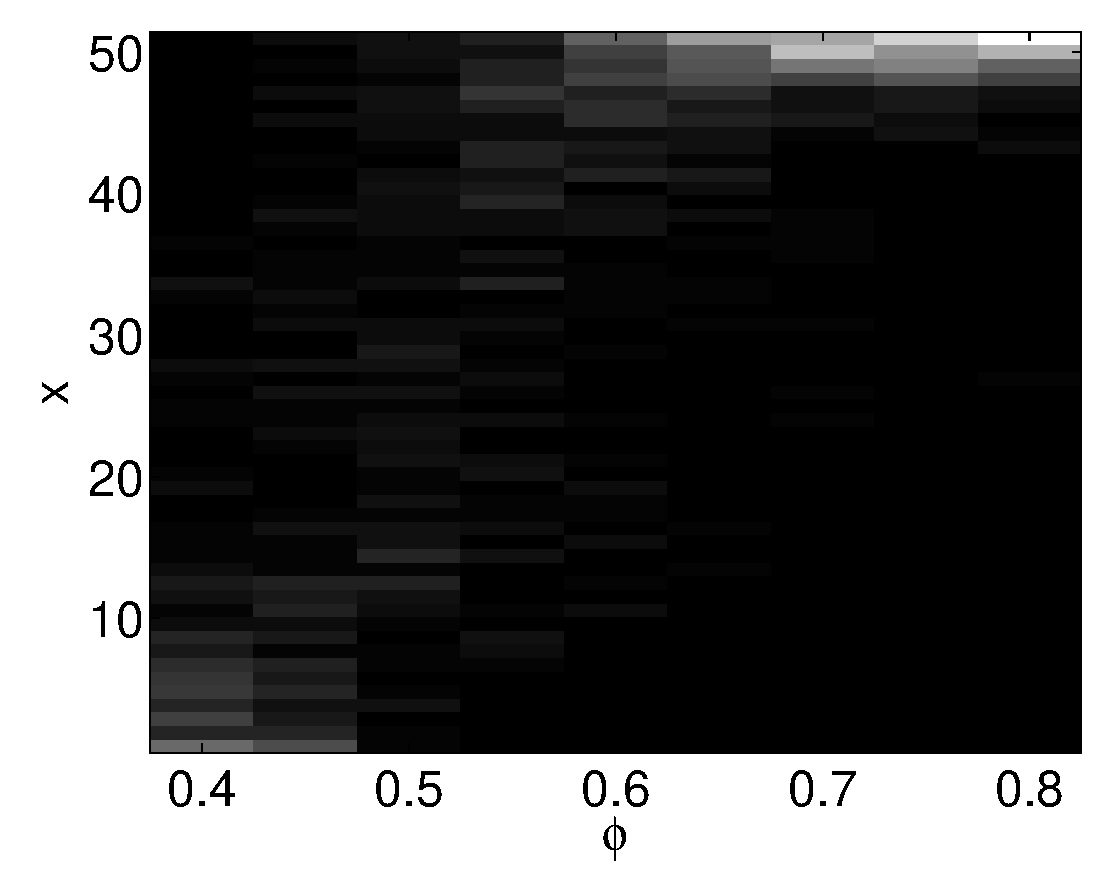
\includegraphics[width=\textwidth]{/home/harrison/Documents/mRNA/Figures_for_writeup/Q_distn_phi.eps}
            \caption[]%
            {{\small Spatial distribution as a function of $\phi$.}}    
            \label{fig:phi}
        \end{subfigure}
        \hfill
        \begin{subfigure}[b]{0.425\textwidth}  
            \centering 
            \includegraphics[width=\textwidth]{/home/harrison/Documents/mRNA/Figures_for_writeup/Q_distn_nu.eps}
            \caption[]%
            {{\small Spatial distribution as a function of $\nu_1$ and $\nu_2$.}}    
            \label{fig:nu}
        \end{subfigure}
        \vskip\baselineskip
        \begin{subfigure}[b]{0.425\textwidth}   
            \centering 
            \includegraphics[width=\textwidth]{/home/harrison/Documents/mRNA/Figures_for_writeup/Q_distn_omega1.eps}
            \caption[]%
            {{\small Spatial distribution as a function of $\omega_1$.}}    
            \label{fig:omega1}
        \end{subfigure}
        \quad
        \begin{subfigure}[b]{0.425\textwidth}   
            \centering 
            \includegraphics[width=\textwidth]{/home/harrison/Documents/mRNA/Figures_for_writeup/Q_distn_omega2.eps}
            \caption[]%
            {{\small Spatial distribution as a function of $\omega_2$.}}    
            \label{fig:omega2}
        \end{subfigure}
        \vskip\baselineskip
        \begin{subfigure}[b]{0.425\textwidth}   
            \centering 
            \includegraphics[width=\textwidth]{/home/harrison/Documents/mRNA/Figures_for_writeup/Q_distn_lambda.eps}
            \caption[]%
            {{\small Spatial distribution as a function of $\lambda$.}}    
            \label{fig:lambda}
        \end{subfigure}
        
        \caption{\small The spatial distribution in the $x$ direction of particles simulated for parameters as in Figure \ref{FIG:Sensitivity_analysis}. For each of (\subref{fig:phi}) to (\subref{fig:lambda}), we vary a parameter in turn. 
        For (\subref{fig:nu}), $\nu_2=\nu_1 /2$ while varying $\nu_1$. Results are shown for 100 particles at time $t=270s$. Note the final spatial box (indexed as box 52) represents particles that have been absorbed and removed from the system.}
        \label{FIG:Sensitivity_of_Q}
    \end{figure*}

In addition, we exhibit the dependence of the spatial distribution parallel to the anterior-posterior axis of particles simulated from our model, as shown in Figure \ref{FIG:Sensitivity_of_Q}.
For increased motor speeds, $\nu_1$ and $\nu_2$, the particles spread out faster from the nucleus and are directed towards the posterior of the nurse cell.
By increasing the microtubule bias, $\phi$, the motion of the cargoes becomes much more directed towards the posterior with accumulation near the posterior and absorption upon reaching the ring canal there.
For high values of the switching rate, $\omega_1$, the distribution of particles is more spread and has not reached the posterior, as little time is spent in the active transport state.
For low values of $\omega_1$, the particles do not change direction often in the active transport state so greater accumulation is seen for intermediate values of $\omega_1$.
We note that, for large values of $\omega_2$, there is an accumulation of particles near the posterior, but that these are not quickly absorbed, since they spend little time in the diffusive phase of motion.
The effect that the turning rate $\lambda$ has on the spatial distribution appears to be unclear.

\subsection{Evaluation of ABC methods for \textit{in silico} data} \label{In_silico}
We demonstrate the effectiveness of the ABC inference techniques on \textit{in silico} data, before applying them directly to real datasets. 
We present first the results of applying ABC methods to our model with a broad prior and known parameter values, as shown in Figure \ref{FIG:ABC_Posterior}.
\begin{figure*} 
        \centering
%        \begin{subfigure}[h]{0.66\textwidth}
%                \includegraphics[width=\columnwidth]{/home/harrison/Documents/mRNA/Figures_for_writeup/Posterior_Scatter_N_2000_RS_v2.png}
%                \caption{Posterior obtained for $N=2000$, $\alpha=0.1$.}
%                \label{fig:a}
%        \end{subfigure}%
        
        
         %add desired spacing between images, e. g. ~, \quad, \qquad, \hfill etc.
          %(or a blank line to force the subfigure onto a new line)
        \begin{subfigure}[h]{0.68\textwidth}
                \includegraphics[width=\columnwidth]{/home/harrison/Documents/mRNA/Figures_for_writeup/Hist_of_posterior_N_2000_RS_from_matlab_v2.png}
                \caption{\small Posterior obtained for $N=2000$, $\alpha=0.1$.}
                \label{fig:b}
        \end{subfigure}
        
          %add desired spacing between images, e. g. ~, \quad, \qquad, \hfill etc.
          %(or a blank line to force the subfigure onto a new line)
        \begin{subfigure}[h]{0.68\textwidth}
                \includegraphics[width=\columnwidth]{/home/harrison/Documents/mRNA/Figures_for_writeup/Pairwise_parameter_heatmap_N2000_RS.png}
                \caption{\small Posterior obtained for $N=2000$, $\alpha=0.1$.}
                \label{fig:c}
        \end{subfigure}
        
        \caption{\small Posterior for each parameter approximated via ABC rejection sampling, using $N=2000$, $\alpha=0.1$, $n_{repeats}=1$. 
        %For \ref{fig:a}, a pairwise scatter plot is shown of all the posterior parameters. 
        In \ref{fig:b}, histograms for each parameter are shown, with a green line for the real parameter values used for the simulated data. For \ref{fig:c}, heatmaps are shown pairwise for the posterior parameters.}
        \label{FIG:ABC_Posterior}
\end{figure*}

For each experiment, we simulate a dataset from chosen parameters and evaluate its summary statistic. 
That summary statistic is compared to summaries of data generated from proposed parameters, as described above.
We average the results obtained across a number of experiments denoted $n_{repeats}$.
As summary statistics we take the spatial distribution of the cargoes averaged in the $x$ direction at given times $t_1,...,t_{\kappa}$ and use a symmetric version of the Kullback-Leibler divergence as our distance to compare distributions.
Broad uniform priors are used for each parameter between biologically realistic maximum and minimum values.
In Figure \ref{FIG:ABC_Posterior}, heatmaps of the pairwise parameter distributions are shown, along with histograms for each parameter. 
%In table (??), we present the results of varying the parameters $N, n_{repeats}, \alpha, p_{acc_{min}}$ on the quality of the posteriors.

We obtain most information from the posterior for the microtubule bias, $\phi$, while the speed parameters, $\nu_1$ and $\nu_2$, are also identifiable. 
The remaining rate parameters have posteriors similar to the uniform prior and it is harder to recover the original parameter values used.
This suggests that the microtubule bias and the speeds have most effect on the summary statistic chosen, which agrees with our earlier sensitivity analysis.
%Explain the set up.
%Which method performs best? Is this consistent?
%Why might this be?

\subsection{Incorporation of production into the model}

Since we have suggested that production is an important part of the mRNA localization process, we choose to examine the effect of incorporating this into our model set out previously in Section \ref{VJ model}.
We assume a constant rate of production, $\gamma$, modelling the export of RNP complexes from the NPC as discrete events that occur as a Poisson process with rate $\gamma$.
Although there is some evidence that the production rate varies during oogenesis, we will assume here that is remains constant for simplification.
Upon export of a particle in our model, it is placed randomly on the circumference of the nucleus and the model evolves as outlined previously.
We begin at time $t=0$ with a single particle that has just been exported, and note that since the production rate is constant 

By introducing the extra parameter, $\gamma$, into our model, there is now an extra parameter to estimate. 
To estimate this directly, we note that rate of production of mRNA is limited by its rate of transcription in the nucleus.
Since the rate of transcription for Drosophila at $22 \degree \text{C}$ is 25 nt/s (BNID 111484) \citep{milo2010bionumbers}, and the length of the \textit{grk} gene is 295 nt \cite{marygold2013flybase}, we can obtain an estimate for the production rate of \textit{grk} mRNA of $\gamma = 0.08 \text{s}^{-1}$.
Simulation from the extended model with production at rate $\gamma=0.08 \text{s}^{-1}$ suggests that a spatial steady state is reached after a short initial transient, with a constant rate of absorption at the posterior ring canal.
Results are shown in Figure \ref{FIG:Production_sim} and exhibit spatial profiles similar to those seen in experimental data exhibited in Figure \ref{FIG:Raw_and_processed_data}.
\begin{figure*}
 \centering
 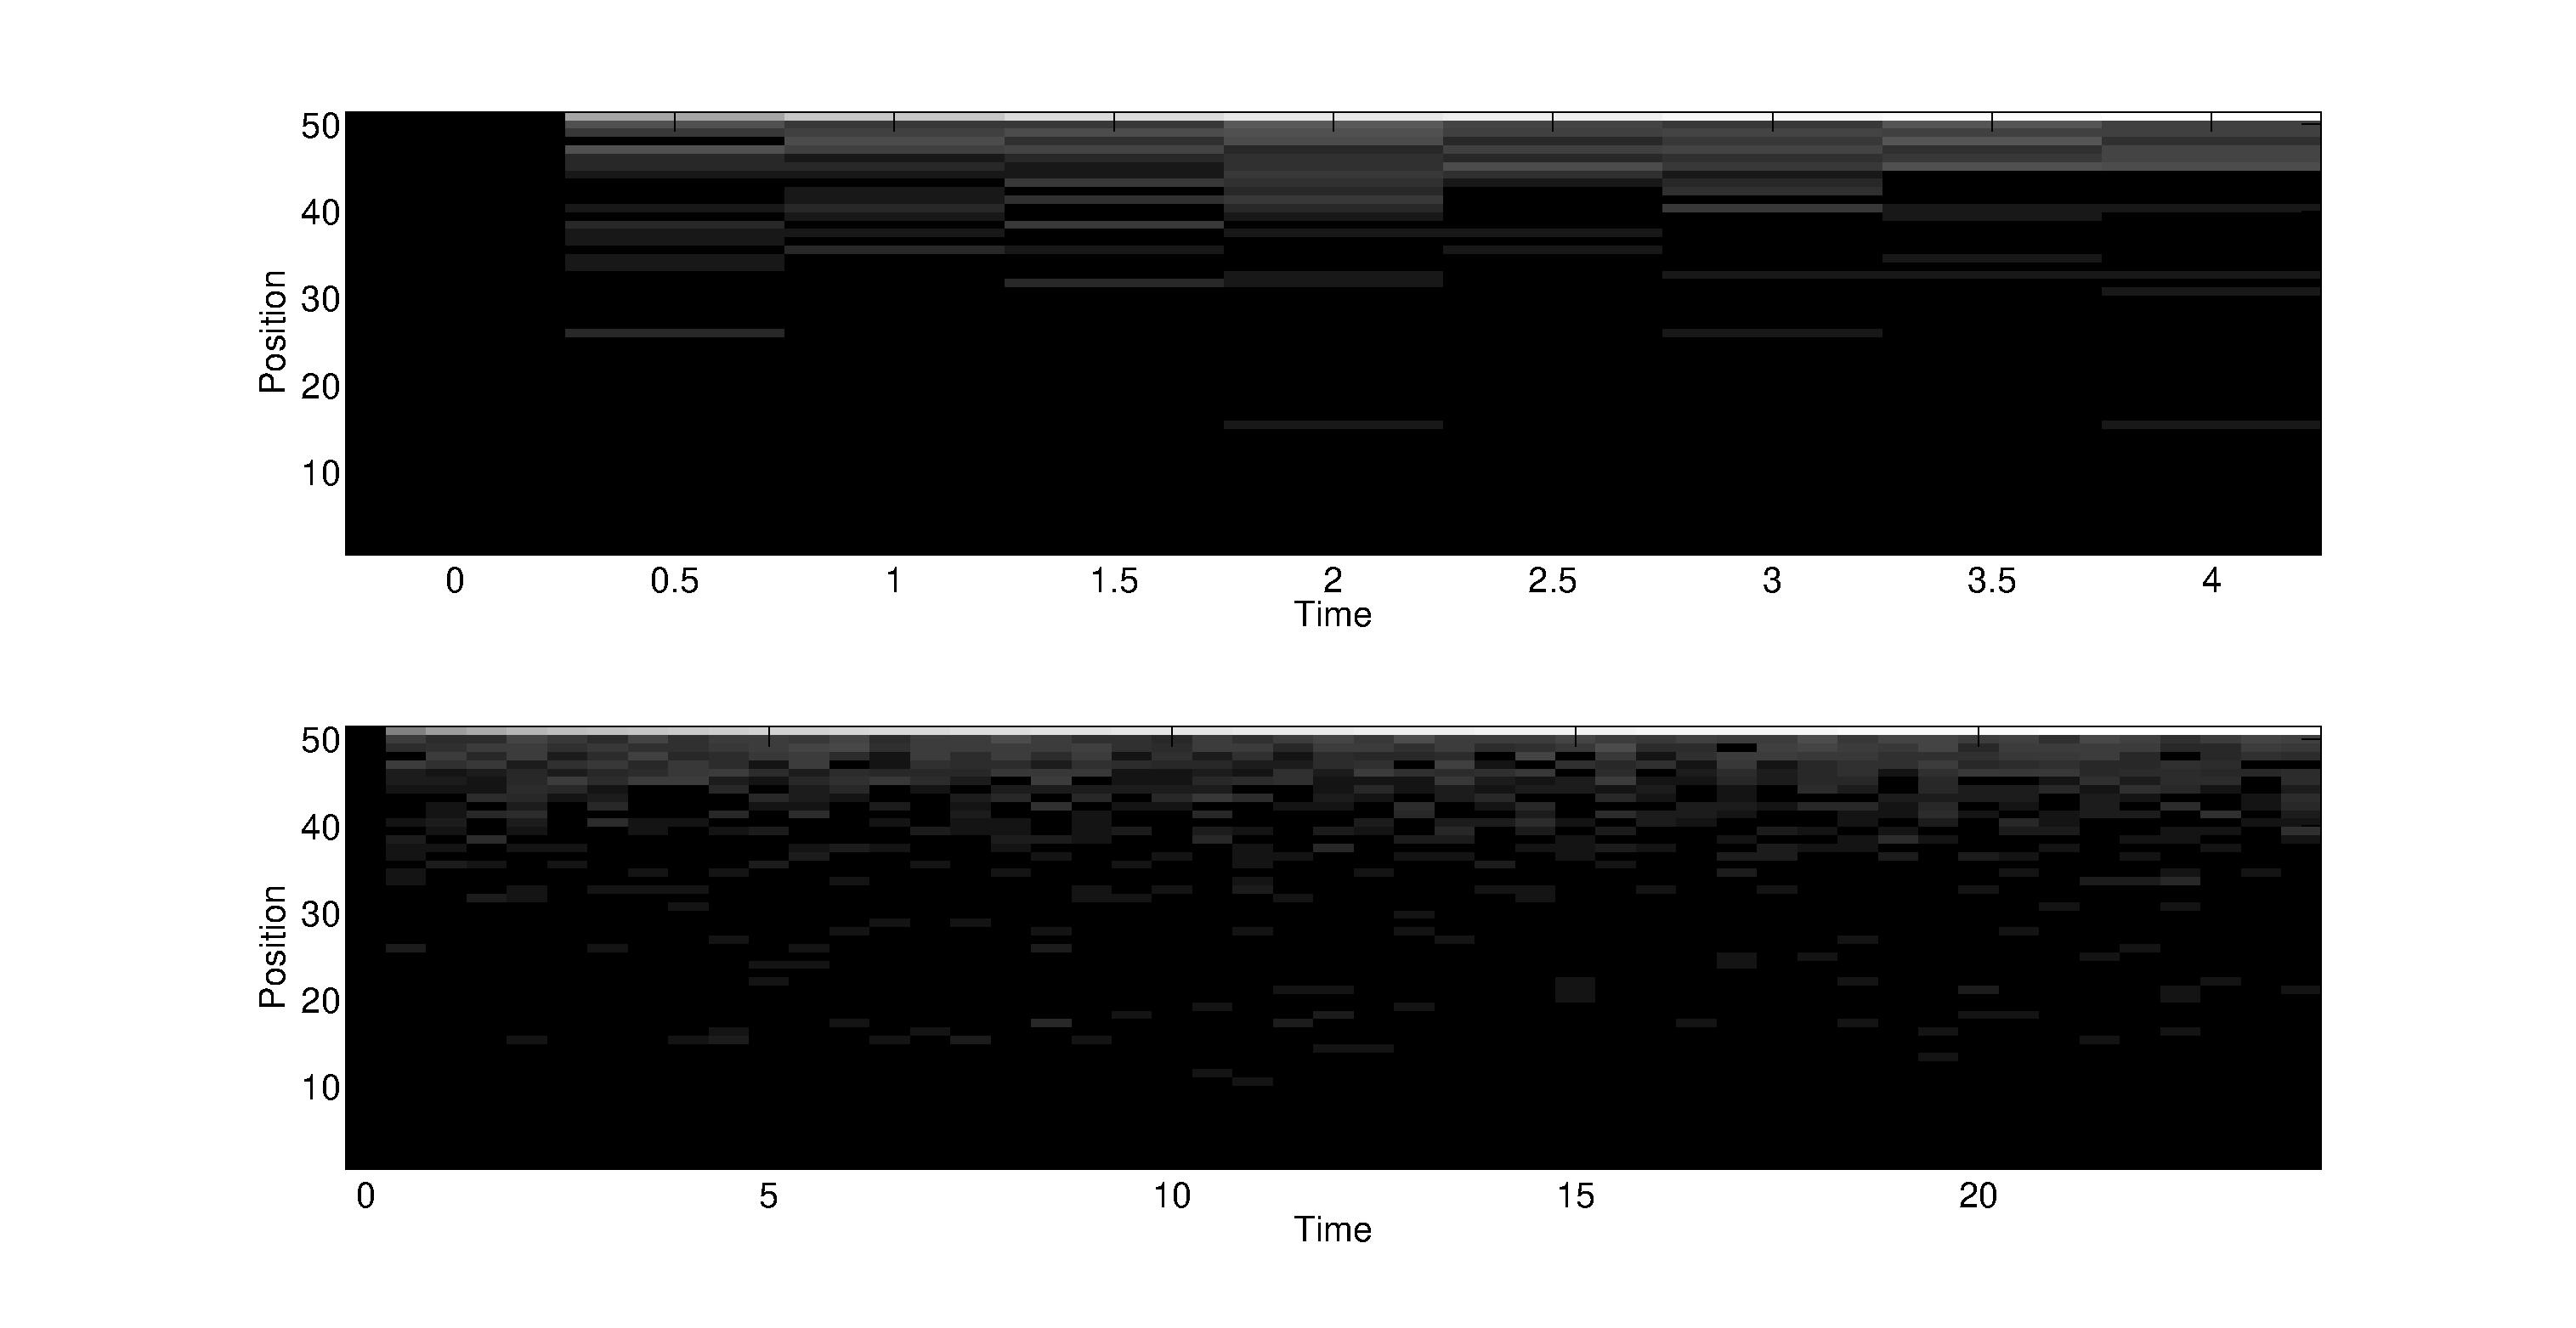
\includegraphics[width = 0.9\textwidth]{/home/harrison/Documents/mRNA/Figures_for_writeup/Spatial_distn_gamma_008.eps}
 \caption{\small The spatial distribution evolving over time up to 25 hours from a single simulation of the model with production included and parameters of $\phi=0.58$, $\nu_1=1.16 \mu \text{ms}^{-1}$, $\nu_2=0.8 \mu \text{ms}^{-1}$, $\omega_1=0.42 \text{s}^{-1}$, $\omega_2=0.84 \text{s}^{-1}$, $\lambda=0.11 \text{s}^{-1}$, $\gamma = 0.08 \text{s}^{-1}$. 
 A logarithmic scale for the colourmap is used to emphasise the presence of small numbers of particles in the nurse cell.}
 \label{FIG:Production_sim}
\end{figure*}

\begin{figure} 
        \centering
        \begin{subfigure}[h]{0.76\columnwidth}
                \includegraphics[width=\columnwidth]{/home/harrison/Documents/mRNA/Figures_for_writeup/Raw_data.jpg}
                \caption{Raw data after denoising and deconvolution.}
                \label{fig:aa}
        \end{subfigure}%
        
        
         %add desired spacing between images, e. g. ~, \quad, \qquad, \hfill etc.
          %(or a blank line to force the subfigure onto a new line)
        \begin{subfigure}[h]{0.86\columnwidth}
                \includegraphics[width=\columnwidth]{/home/harrison/Documents/mRNA/Figures_for_writeup/Processed_data.eps}
                \caption{Spatial distribution of \textit{grk} particles seen in raw data.}
                \label{fig:bb}
        \end{subfigure}
        
        \caption{\small Distribution of \textit{grk} MCP Dendra in a stage 5 \text{Drosophila} oocyte and surrounding nurse cells. Stage 5 is equivalent to a time point of around $t=25$ hours, assuming \textit{grk} mRNA production begins at stage 2. A logarithmic scale for the colourmap is used in (\subref{fig:bb}).}
        \label{FIG:Raw_and_processed_data}
\end{figure}

\subsection{Application of ABC to \textit{Drosophila} nurse cell data}
%We collected some data.
%What did we collect? Why? Might it have been more informative if we could have collected something else?
%Why didn't we do that?
%What estimates for the posterior of the parameters do we get from ABC?
%Are these informative?
%Do they agree with what we obtained by direct measurement? Why?
Although comparative simulation results with ABC suggest that the detailed summary statistics using MFPT, number of jumps and jump distances result in a higher quality posterior, there are limitations to what data can be collected experimentally.
In particular, these summary statistics would require detailed tracking data of individual particles over an extended period of time, which would be difficult to obtain. 
Instead, we use the spatial distribution of particles which is more tractable from a single time point.
To ensure the timescales of the observed experimental data and simulated data match, we use the model with production of mRNA at rate $\gamma$ and infer this parameter also.

Applying inference with ABC to these data using a Euclidean distance measure and binned spatial histograms in the $x$ direction as summary statistics, we obtain posteriors for the model parameters as shown in Figure \ref{FIG:ABC_real_data}.
Since simulating from the model with production over longer timescales is more computationally intensive than simulating from the original model, as in Section \ref{In_silico}, we must sample fewer parameter values, taking $N=500$ and $\alpha=0.1$ in the ABC rejection sampling algorithm.
The results of the ABC inference show a very tight distribution for $\gamma$, despite the low value of $N$ used in these simulations. 
This suggests that the output of the production model depends most strongly on $\gamma$ when summarised by our chosen summary statistics.
Little extra information beyond the prior is gained for the other parameters, based on these results with $N=500$.
\begin{figure*} 
        \centering
        \begin{subfigure}[h]{0.66\textwidth}
                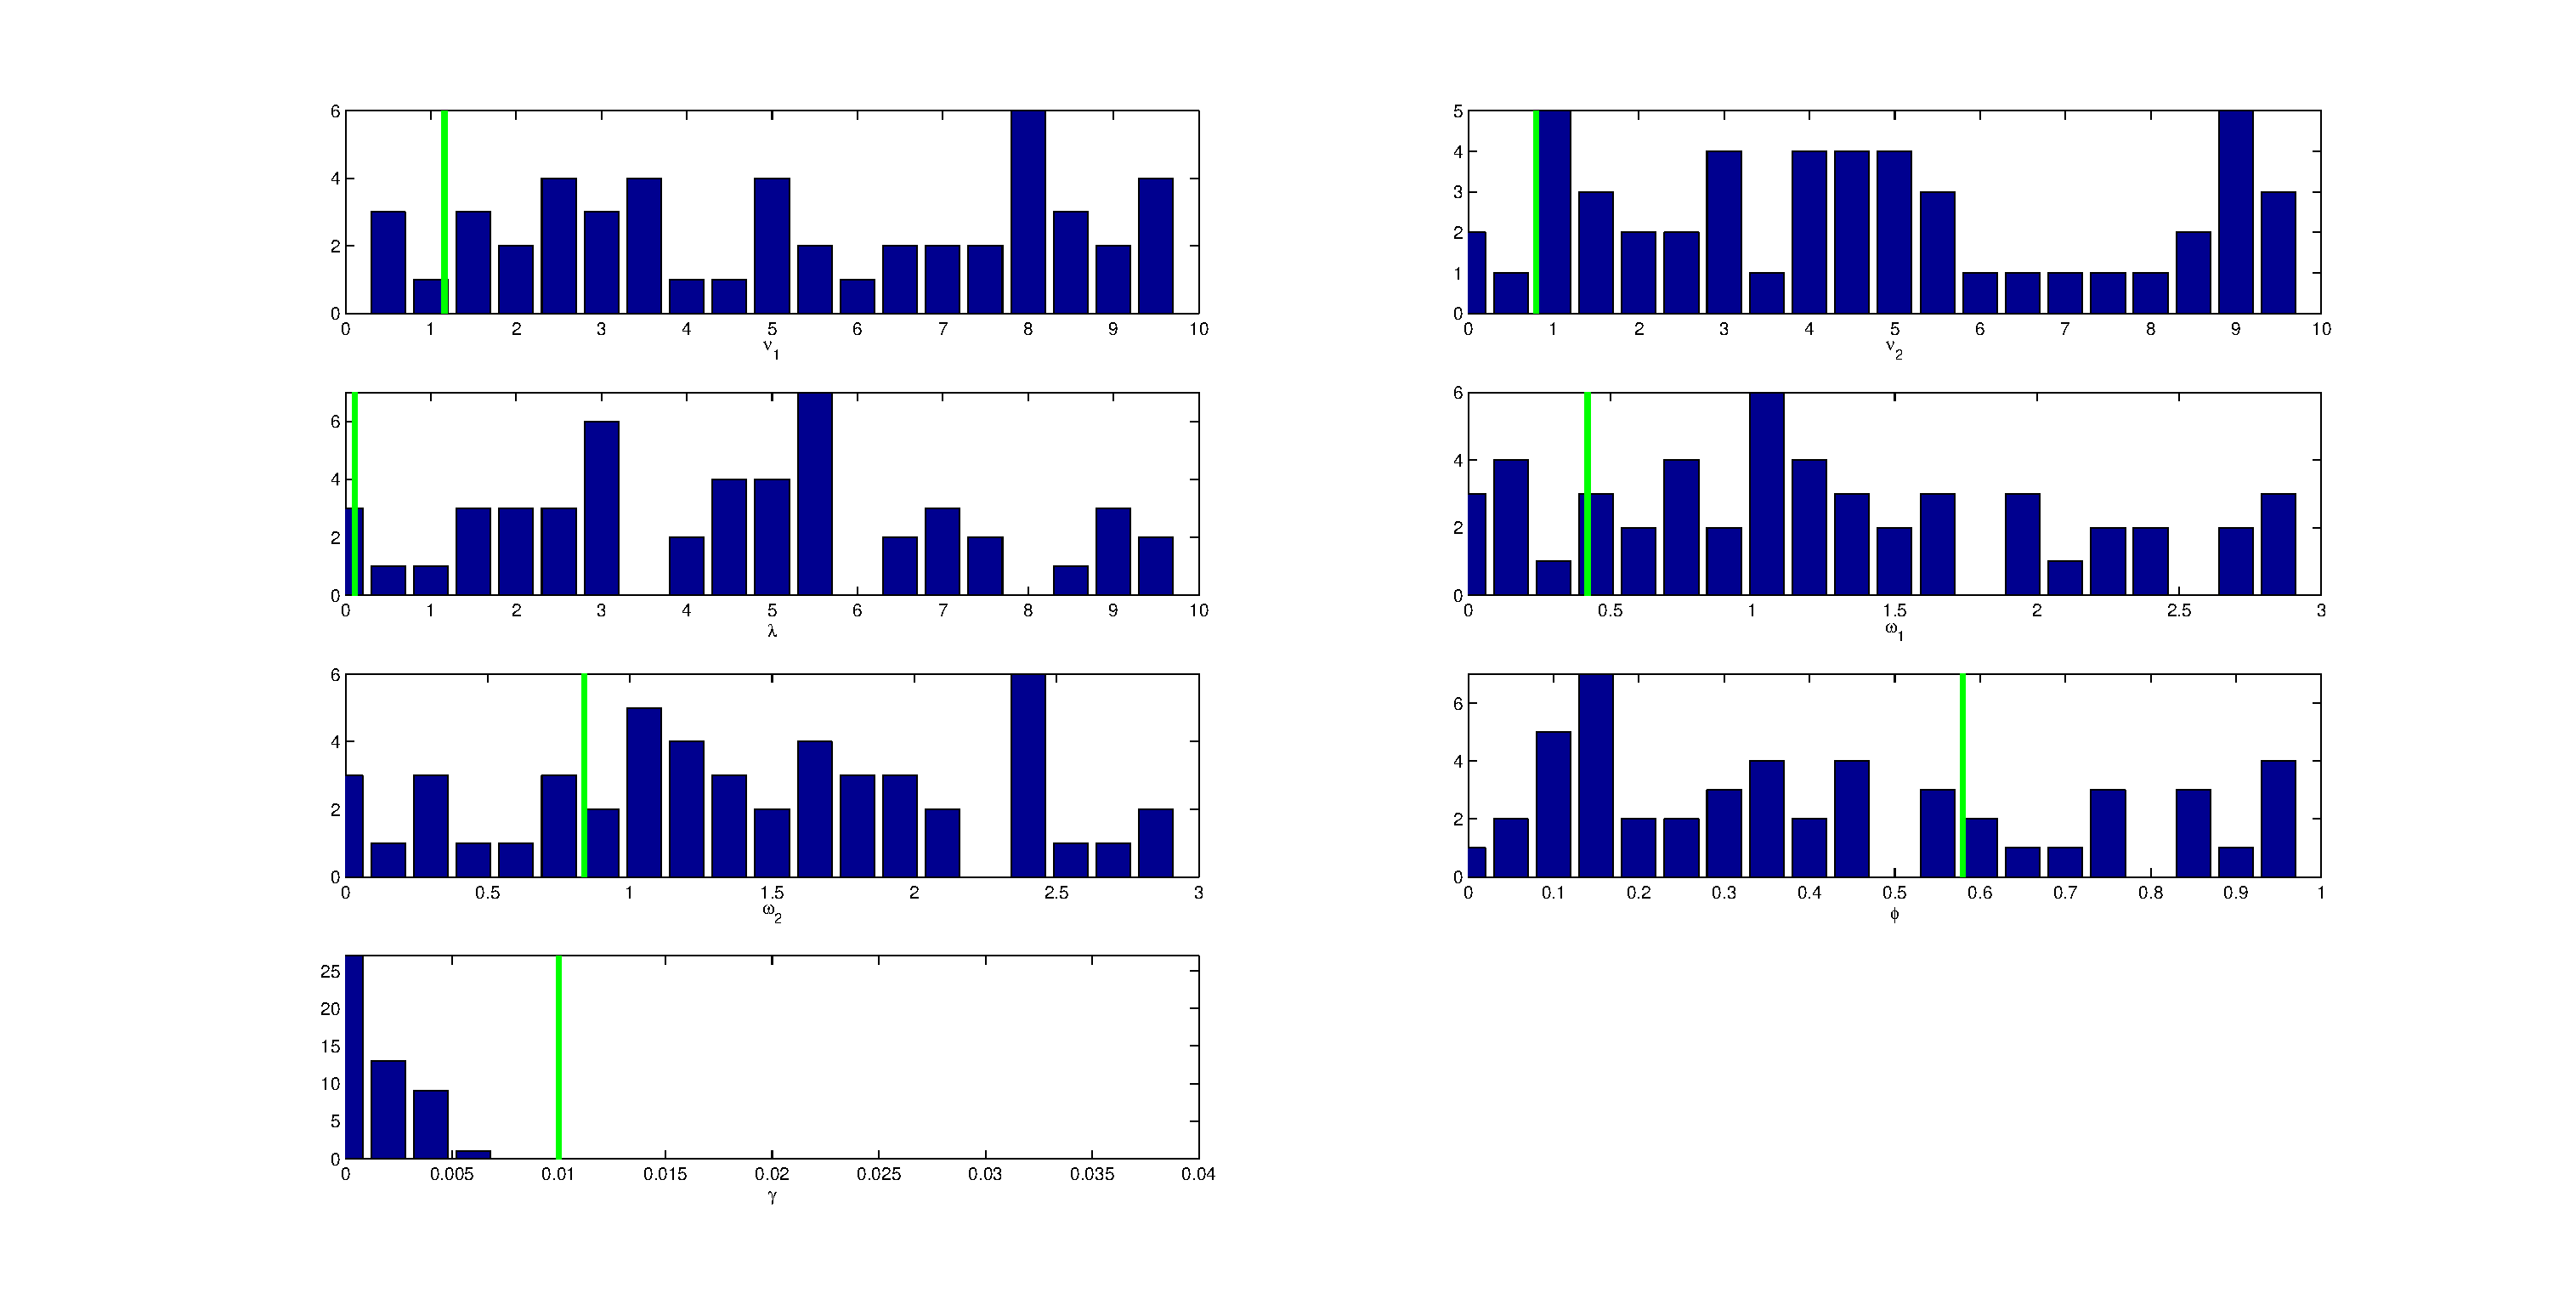
\includegraphics[width=\columnwidth]{/home/harrison/Documents/mRNA/Figures_for_writeup/Auto_hist_w_production2.eps}
                \caption{Histogram for each parameter.}
                \label{fig:hist}
        \end{subfigure}%
        
        
         %add desired spacing between images, e. g. ~, \quad, \qquad, \hfill etc.
          %(or a blank line to force the subfigure onto a new line)
        \begin{subfigure}[h]{0.76\textwidth}
                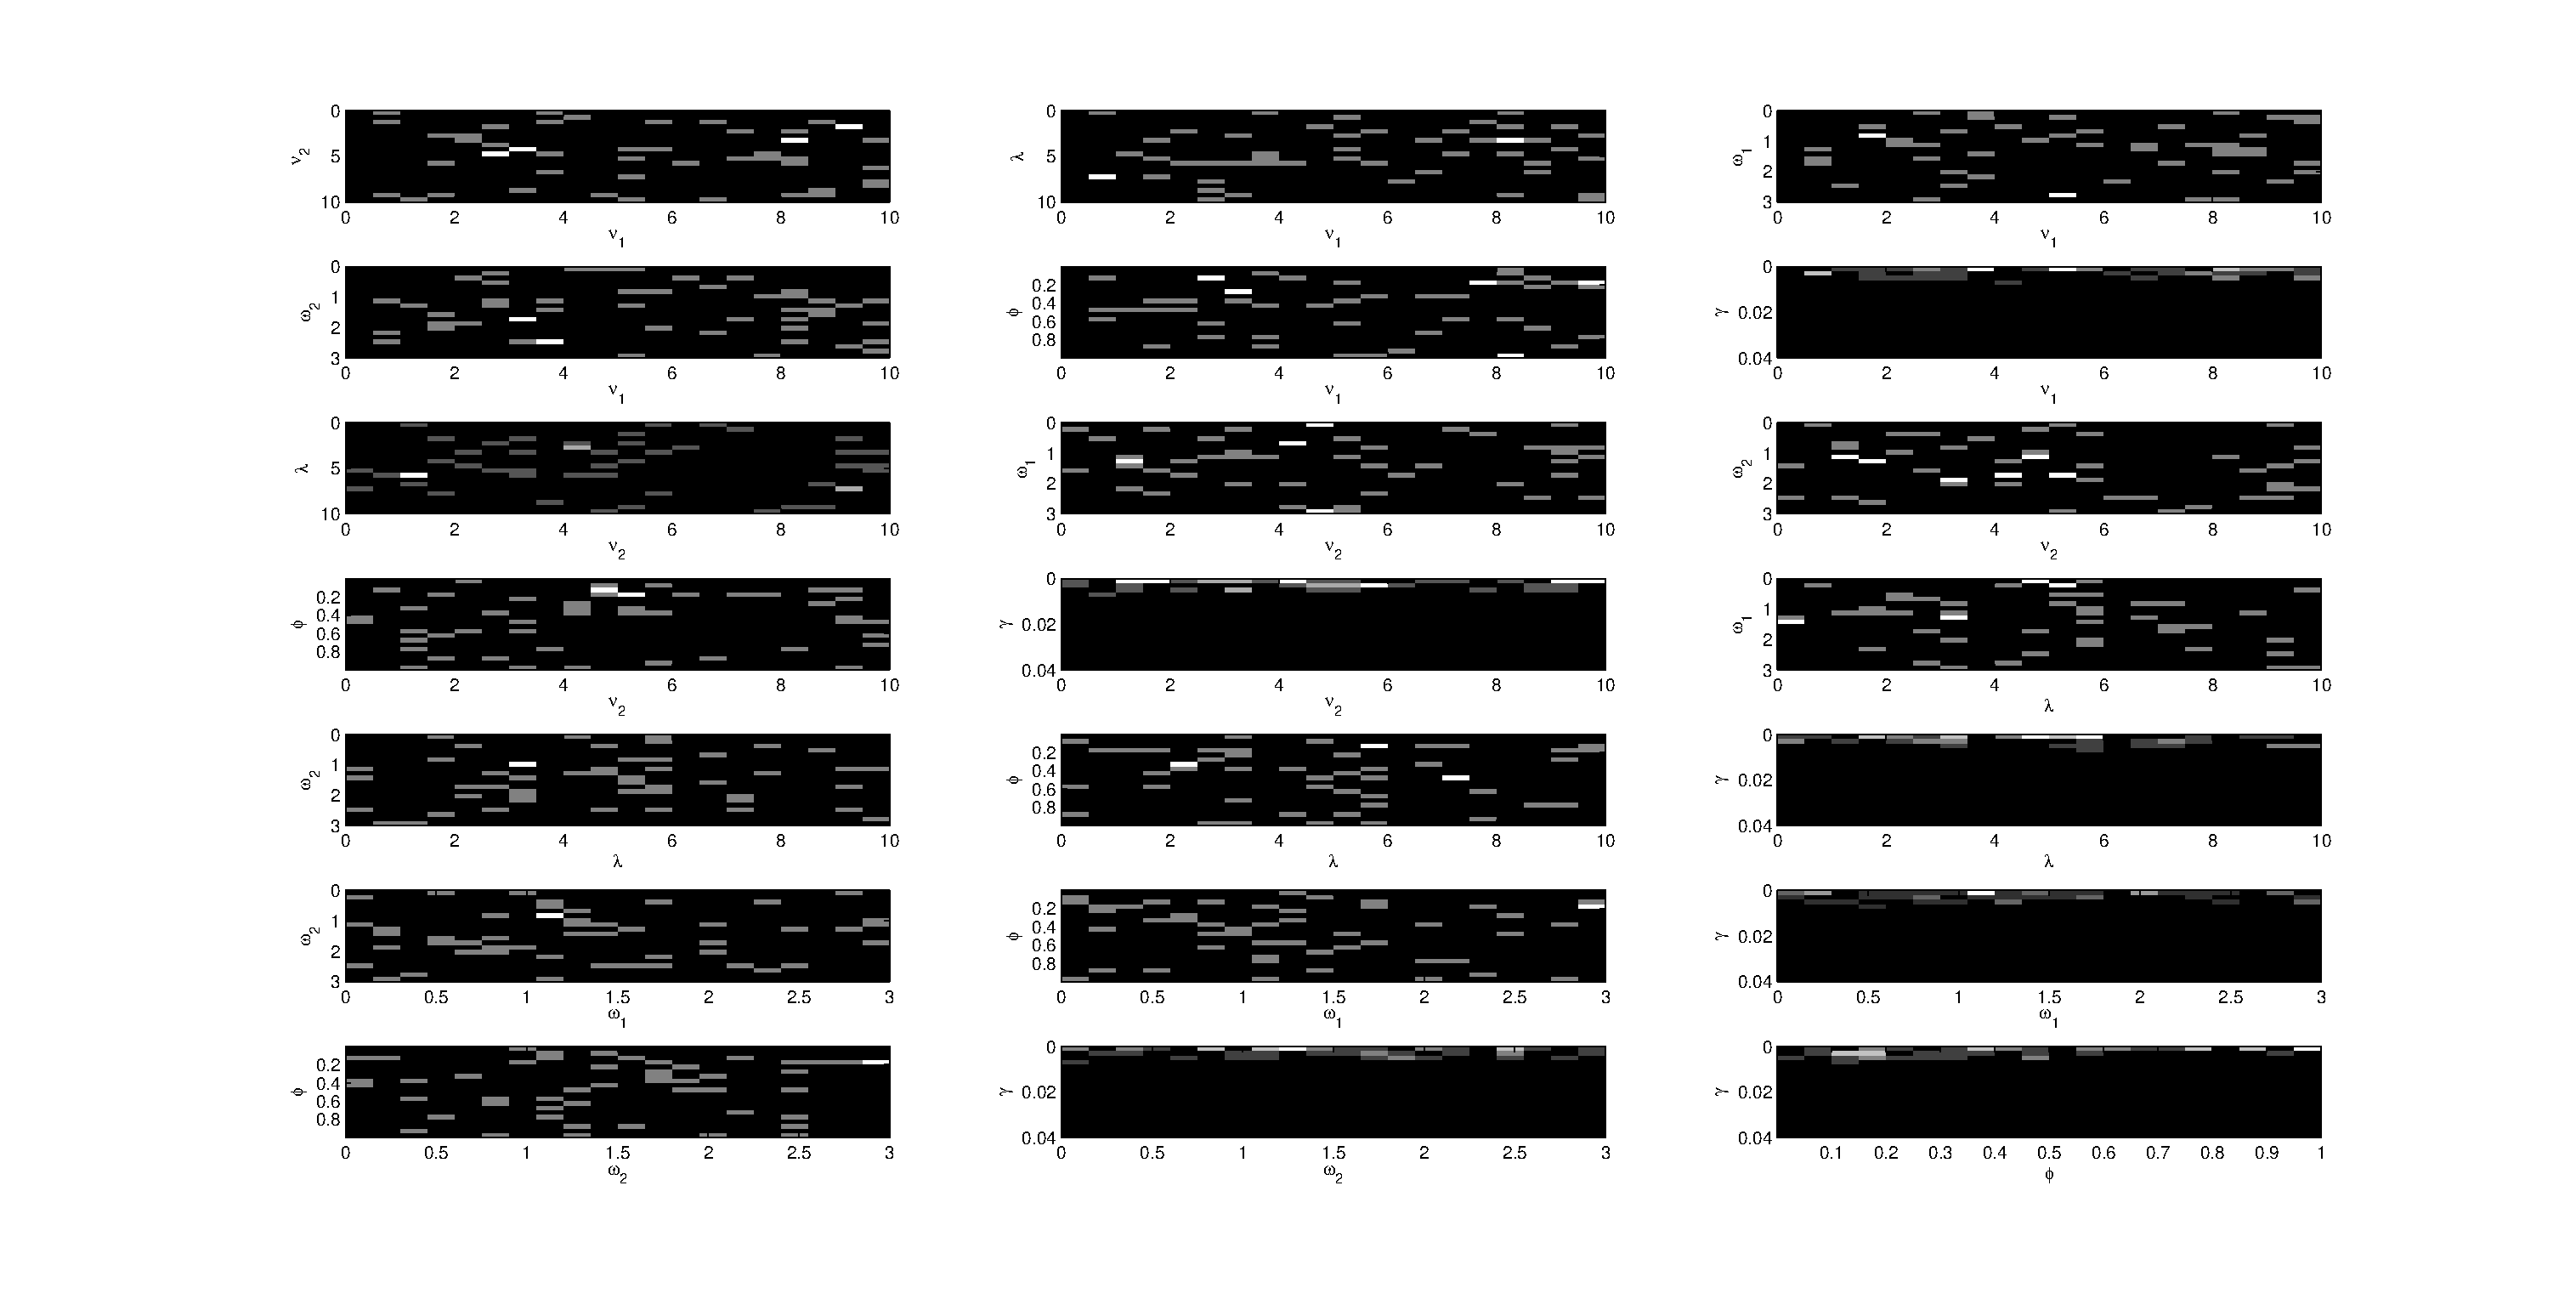
\includegraphics[width=\columnwidth]{/home/harrison/Documents/mRNA/Figures_for_writeup/Auto_heatmap_w_production2.eps}
                \caption{Heatmap for pairwise parameters.}
                \label{fig:heat}
        \end{subfigure}
        
        \caption{\small Posterior for each parameter in the full model with production approximated via ABC rejection sampling, using $N=500$, $\alpha=0.1$, based on real data from one single image frame. 
        In \ref{fig:hist}, histograms for each parameter are shown, with a green line for the directly estimated parameter values  for comparison. For \ref{fig:heat}, heatmaps are shown pairwise for the posterior parameters.}
        \label{FIG:ABC_real_data}
\end{figure*}

\section{Conclusion} \label{Conclusions}
Through use of a model-based approach for explaining mRNA transport and localization, we have been able to represent the dynamics of this process and reproduce behaviour observed experimentally, showing that a biased network of microtubules can maintain localization of mRNA.
We constructed a velocity jump process with two phases of motion to represent directed movement via active transport on microtubles and random motion in free diffusion.
Since simulations of this model were accessible but the likelihood was intractable, we employed ABC methods to infer the parameters from our model from data collected via live \textit{in vitro} imaging and compared the results of this with values obtained from direct measurement.

The timescales for MFPTs based on simulations from the model are on the order of tens of minutes, rather than hours, for the inferred parameters, suggesting that the transport step is not the rate-limiting stage of the mRNA localization process.
Based on the modelling work presented here, we postulate that the production of mRNA in the nucleus of the nurse cells is instead the rate-limiting stage.

By incorporating production at a constant rate into our model, we recover transport on timescales of the order of hours seen during oogenesis.
We are also able to simulate spatial distributions of mRNA particles similar to what is observed experimentally.  

\subsection{Further work}
The subcellular environment is in many ways drastically different to that assumed in our spatially homogeneous two-dimensional model.
In reality, cells exist in three dimensions and are crowded inside with a heterogeneous environment. 
One possible method of representing heterogeneity in the cell would be by use of a potential to account for volume exclusion effects, as used by \citet{isaacson2011influence} in the context of nuclear export of mRNAs.
The three-dimensional nature of the environment presents further challenges for tracking, as RNPs move between frames.
Although some progress has already been made in this area \citep{thompson2010three}, we hope that incorporation of modelling into a tracking framework could enable tracking of particles over longer timescales at increased resolution. 
Motivated by a Kalman filter type approach \citep{faragher2012understanding}, we hope to investigate further using our model combined with regular inputs of data over time to assist particle tracking algorithms in the linkage step of tracking.
Therefore in future the model should be extended to enable us to capture behaviour in three dimensions. 
Since the oocyte more than triples in size during the early stages of oogenesis, it may be relevant to include domain growth in our model in future, as the dimensions of the domain effect the timescales of the MFPT of the process.

If further time were available, we would investigate further the parameterization of the full model from experimental data via ABC, which may require use of other ABC algorithms, such as Adaptive Population Monte Carlo ABC \citep{lenormand2013adaptive}, to overcome the inefficiencies of the rejection sampling method.
We could compare more comprehensively a variety of summary statistics to guide the use of experiments in inference of our model parameters.
%Furthermore, it would be beneficial to examine quantitatively the agreement between our simulated results using the model with production and experimental data to provide model validation.
%If further time were available, we would seek to parametrise this full model from experimental data via ABC. 

\section*{SUPPLEMENTARY MATERIAL}

\ack{Two Sections and one Figure are available as a supplement to this article below and can be found by visiting BJ Online at http://www.biophysj.org.}

\vspace{1cm}
%\footnotesize 
\ack{The authors would like to acknowedge valuable discussions with Dr S. Filippi and Dr J. Rittscher.}

\appendix

\section{Further sensitivity analysis} \label{Sensitivity_analysis_2}
\normalsize
Here, we show, in Figure \ref{FIG:Sensitivity_analysis_2}, the sensitivity of the mean number of jumps per simulation and the mean of the median jump distance to the parameters of the basic model without production. 
	\begin{figure*}
        \centering
        \begin{subfigure}[b]{0.425\textwidth}
            \centering
            \includegraphics[width=\textwidth]{/home/harrison/Documents/mRNA/Figures_for_writeup/Two_sum_stats_phi.eps}
            \caption[]%
            {{\small Microtubule bias, $\phi$.}}    
            \label{fig:3phi}
        \end{subfigure}
        \hfill
        \begin{subfigure}[b]{0.425\textwidth}  
            \centering 
            \includegraphics[width=\textwidth]{/home/harrison/Documents/mRNA/Figures_for_writeup/Two_sum_stats_nu.eps}
            \caption[]%
            {{\small Motor speeds, $\nu_1$ and $\nu_2$.}}    
            \label{fig:3nu}
        \end{subfigure}
        \vskip\baselineskip
        \begin{subfigure}[b]{0.425\textwidth}   
            \centering 
            \includegraphics[width=\textwidth]{/home/harrison/Documents/mRNA/Figures_for_writeup/Two_sum_stats_omega1.eps}
            \caption[]%
            {{\small Switching rate to diffusion, $\omega_1$.}}    
            \label{fig:3omega1}
        \end{subfigure}
        \hfill
        %\quad
        \begin{subfigure}[b]{0.425\textwidth}   
            \centering 
            \includegraphics[width=\textwidth]{/home/harrison/Documents/mRNA/Figures_for_writeup/Two_sum_stats_omega2.eps}
            \caption[]%
            {{\small Switching rate to active transport, $\omega_2$.}}    
            \label{fig:3omega2}
        \end{subfigure}
        \vskip\baselineskip
        \begin{subfigure}[b]{0.425\textwidth}   
            \centering 
            \includegraphics[width=\textwidth]{/home/harrison/Documents/mRNA/Figures_for_writeup/Two_sum_stats_lambda.eps}
            \caption[]%
            {{\small Reorientation rate in diffusion, $\lambda$.}}    
            \label{fig:3lambda}
        \end{subfigure}
        
        \caption{ \small Dependence of the number of jumps and the length of jumps on the model parameters. Parameters used for simulations were $\phi=0.58$, $\nu_1=1.16 \mu \text{ms}^{-1}$, $\nu_2=0.8 \mu \text{ms}^{-1}$, $\omega_1=0.42 \text{s}^{-1}$, $\omega_2=0.84 \text{s}^{-1}$, $\lambda=0.11 \text{s}^{-1}$.
        For each of (\subref{fig:3phi}) to (\subref{fig:3lambda}), we vary each parameter in turn. 
        For (\subref{fig:3nu}), $\nu_2=\nu_1 / 2$ while varying $\nu_1$. Results are averaged over 100 particles with standard deviation shown on the error bars.}
        \label{FIG:Sensitivity_analysis_2}
    \end{figure*}

    \section{Analytics}
%\subsubsection{Analytics}
For many models, analytical techniques can offer more general insight than simulating from the model with specific parameters.
We show here what can be achieved with these techniques and give some indicative results.
First, we must make some simplifying assumptions to ensure the model is analytically tractable. We will consider only one spatial distribution on the interval $[0,L_x]$, parallel to the $x$ axis.
Furthermore, we assume $\nu_1 \gg \nu_2$ so that it is reasonabe to ignore the diffusive phase of motion, leaving only reorientations with the active transport phase at rate $\omega_1$.

Suppose we have a velocity jump process with one mode of motion in one dimension where the speed in the $x$ direction varies as $\nu_1 \sin (\theta)$ when the velocity is oriented in direction $\theta$ in two dimensions.
Let $ p(x,\theta,t | y, \alpha, s)\text{d}t$ be the probability that the particle is at position $x$ moving in direction $\theta$ in the time interval $[t,t+dt)$ having started previously at time $s$ at position $y$ moving in direction $\alpha$.
We will now suppress the conditioning and write only $ p(x,\theta, t) $.

The evolution of the probability is governed \citep{othmer1988models} by :
\begin{equation}\label{Evolution}
 \frac{\partial p}{\partial t} + \nu_1 \sin{\theta } \frac{\partial p}{\partial x} = -\omega_1 p + \omega_1 \int_0^{2\pi} T(\theta) p(x,\theta ', t) \text{d} \theta ',
\end{equation}
where the turning kernel $T(\theta)$ gvies the probability of reorienting into a new angle $\theta$ and we assume this does not depend on the previous angle.
We define $\mean{f(\theta)} = \int_0^{2\pi} f(\theta) \text{d} \theta $ and $\mean{\mean{f(x,\theta)}} =  \int_{0}^{2\pi} \int_0^{2\pi} f(\theta) \text{d} \theta \text{d}  x $.

The orientation of the velocity, $\theta$, is updated via the reorientation kernel $T(\theta)$ after every transition.
It depends only on the initial condition and the kernel $T(\theta)$.
After a sufficiently long time, the initial condition will have been forgotten and we should be able to decompose the probability $p$ such that:
\begin{equation}\label{decomposition}
 p(x,\theta , t) = T(\theta) q(x,t),
\end{equation}
since whenever the angle $\theta$ is updated, this is independent of time or position. 
For a particle to forget the initial condition, it must simply execute at least one jump. 
After a time $t_{\text{min}} = 1/\omega_1 \log (100)$, then $99\%$ of the particles should have executed a jump, since this is the 99th percentile of an exponential distribution with parameter $\omega_1$.
Assuming a value of $\omega_1 = 0.42 \text{s}^{-1}$, then $t_{\text{min}} = 11 \hspace{0.5mm} \text{s}$ which is much less than our timescales of interest. 

Now integrating \eqref{Evolution} over $\theta$, we obtain:
\begin{equation}
 \frac{\partial}{\partial t} \mean{p} + \frac{\partial}{\partial x} \mean{\nu_1 \sin(\theta) p} = 0,
\end{equation}
which becomes via our assumption \eqref{decomposition}: 
\begin{equation}
 \frac{\partial q}{\partial t} + \nu_1 \mean{T(\theta) \sin(\theta)} \frac{\partial q}{\partial x} = 0.
\end{equation}

From multiplying by $x$ and considering the first spatial moment, we have:
\begin{align*}
 \frac{\partial}{\partial t} ( \mean{\mean{x p}} & = \nu_1 \mean{\mean{\sin{\theta} p}}, \\
 \frac{\partial}{\partial t} ( \mean{\mean{x T(\theta) q}} & = \nu_1 \mean{\mean{\sin{\theta} T(\theta) q}}, \\
 %\frac{\parequationtial}{\partial t} ( \int_0^L x q \text{d} x ) & = \nu \mean{\sin{\theta} T(\theta) } \int_0^L q \text{d} x, \\
 \frac{\partial}{\partial t} \left( \int_0^L x q \hspace{1mm} \text{d} x \right) & = \nu_1 \mean{\sin{\theta} T(\theta) } \int_0^L q \hspace{1mm} \text{d} x.
 \end{align*}
Suppose we let $\mu^{(1)}(t) = \int_0^L x q(x,t) \text{d} x  $. Then we can write:
\begin{align}
 \frac{\text{d} \mu^{(1)}}{\text{d} t} &= \nu_1 \mean{\sin(\theta) T(\theta)} \int_0^L q \hspace{1mm} \text{d} x, \nonumber \\
 \mu^{(1)}(t) &= \mu^{(1)}(0) + \nu_1 \mean{\sin(\theta) T(\theta)} \int_0^t \int_0^L q \hspace{1mm} \text{d} x \text{d} t.
\end{align}
We can interpret $\int_0^L q(x,t) \hspace{1mm} \text{d} x$ as a survival probability of a particle at time $t$.
After very short times, when the particle cannot physically have exited the system yet, this will equal one, leading to a linear form for the average position, $\mu^{(1)}(t)$. 
At later times, the particle may have exited the system and the survival probability will decrease to 0.
If we release an ensemble of particles, the average position of this ensemble changes according to the mean net velocity, $\nu_1 \mean{\sin(\theta) T(\theta)}$, until particles begin to be absorbed.
We note that this mean net velocity depends on the microtubule bias. 
For our specified choice of $T(\theta)$, we have $\nu_1 \mean{\sin(\theta) T(\theta)} = \nu_1 (4 \phi -2)/\pi$.
Using our estimated parameters, $\phi=0.58$ and $\nu_1 = 1.16 \mu \text{ms}^{-1}$, we find an estimate of the mean net velocity of $0.12 \mu \text{ms}^{-1}$.

By similar arguments, expressions for higher spatial moments and angular moments can be obtained.
For the $j$th spatial moment, we have
\begin{equation}
 \frac{\partial \mu^{(j)}}{\partial t} = j \nu_1 \mean{\sin(\theta) T(\theta)} \mu^{(j-1)}, 
\end{equation}
leading to a hierarchy of equations.
Extensions of these arguments to the full model with two phases of motion are also possible. 



% Here references are directly included this tex file.
% But we can generate reference list from bibliography database
% Compile and format the bibliography (bj_bibtex_template.bib BibTeX
% file must be present in the document directory)

%The source file for this document is called
%\emph{biophys\_latex\_template.tex}.  Apart from this \LaTeX\ file, you
%will also need the bibliography file, the \BibTeX\ style file, and the
%EPS and PDF figure files.

%See the bibliography file \emph{bj\_bibtex\_template.bib} for the
%literature data.  It was mostly generated from the saved
%text-formatted PubMed entries using the \emph{med2bib} program and
%edited by the \emph{tkbibtex} or directly in the \emph{emacs} editor.

%The \emph{biophysj.bst} file is a \BibTeX\ style file that contains
%information about the format required by Biophysical Journal for the
%list of references.


%\bibliography{bj_bibtex_template}

% Bibliography style (requires the style file biophysj.bst in the
% document directory)
\bibliographystyle{biophysj}
\bibliography{my_citations.bib}

% Figure legends
%%Automatically it will add the figure legends  and table legends as a list by below command


%\newpage

%\listoffigures

%\newpage

%\listoftables

% Figures and Tables coding should be placed where the
% first reference in the text.
% All the Figure files should be placed same working directory,
% for example (fig_1.eps and fig_1.pdf files must be present
% in the document directory)

% closing statement, nothing below matters

\end{document}




%%%%%%%%%%%%%%%%%%%%%%%%%%%%%%%%%%%%%%%%%%%%%%%%%%%%%%%%%%%%%%%%%%%%%%%%%%%%%%%%%%%%%%%%%%%%%%%%%%%%%%%%%%%%%%%%%%%%%%%%%%%%%%%%%%%%%%%%%%%%%%%%%%
%This has been placed after the end of the document because we have not successfully used the ABC_APMC algorithm in this work.
This is implemented as shown in Algorithm \ref{ABC-APMC}, where $N$ is the number of parameter samples to simulate, $N_{\alpha} = \floor{\alpha N}$ is the number to keep at each iteration, $p_{acc_{min}}$ is the minimum acceptance rate at which the algorithm stops, and a Gaussian kernel $K_{\sigma}(x,y)$, where:
$$K_{\sigma}(x,y) = \frac{1}{\sqrt{2\pi \sigma^2}} e^{-\frac{(x-y)^2}{2\sigma^2}}.$$
\begin{algorithm}
\caption{ABC Adaptive Population Monte Carlo}\label{ABC-APMC}
\begin{algorithmic}[1]
\State Initialise by setting $N$,$\alpha$, $N_{\alpha}$ and $p_{acc_{min}}$.
\State Set $t=1$.
\State \textbf{for} $i=1$ \text{to} $N$  \{
\State Sample form prior: $\theta \sim \pi (\theta)$. 
\State Simulate data $x \sim f \left(x|\theta_i^{(0)} \right)$.
\State Calculate distance from observed data $y$ via $\rho_i^{(0)} = \rho(S(x),S(y))$
\State Set $w_i^{(0)} = 1$.
\State \}
\State Take $\epsilon_1$ as the first $\alpha$-quantile of $\rho^{(0)}$.
\State Let \{ $(\theta_i^{(1)},w_i^{(1)}, \rho_i^{(1)})$ \} = \{ $(\theta_i^{(0)},w_i^{(0)}, \rho_i^{(0)}) | \rho_i^{(0)} \le \epsilon_1, 1 \le i \le N$ \} 
\State Take $\sigma_1^2$ as twice the weighted empirical variance of $\{(\theta_i^{(1)} ,w_i^{(1)}) \} _{1\le i \le N_{\alpha}}$
\State Set $p_{acc} = 1$.
\State Update $t:=t+1$
\State \textbf{while} $p_{acc}>p_{acc_{min}}$ \{ 
\State \textbf{for} $i=N_{\alpha+1}$ \text{to} $N$ \{
\State Pick $\theta_i^{*}$ from $\theta_j^{(t-1)}$ with probability $\frac{\omega_j^{(t-1)}}{\sum_{k=1}^{N_{\alpha}} w_k^{(t-1)}  }$, $1 \le j \le N_{\alpha}$.  
\State Generate new parameters $\theta_i^{(t-1)}|\theta_i^{*} \sim \mathcal{N} \left(\theta_i^{*}, \sigma_{(t-1)}^2 \right)$ and data $x \sim f \left(x|\theta_i^{(t-1)} \right)$
\State Set$ \rho_i^{(t-1)} = \rho (S(x),S(y))$
\State Set $w_i^{(t-1)} = \frac{\pi(\theta_i^{(t-1)}}{\sum_{j=1}^{N_{\alpha}}(w_j^{(t-1)}/\sum_{k=1}^{N_{\alpha}} w_k^{(t-1)}) K_{\sigma_{(t-1)}}\left(\theta_i^{(t-1)},\theta_j^{(t-1)} \right) }$
\State \}
\State Set $p_{acc} = \frac{1}{N-N_{\alpha}} \sum_{k=N_{\alpha}+1}^N \mathds{1}_{\rho_i^{(t-1)} < \epsilon_{t-1}}$
\State Take $\epsilon_1$ as the first $\alpha$-quantile of $\rho^{(t-1)}$.
\State Let \{ $(\theta_i^{(t)},w_i^{(t)}, \rho_i^{(t)})$ \} = \{ $(\theta_i^{(t-1)},w_i^{(t-1)}, \rho_i^{(t-1)}) | \rho_i^{(t-1)} \le \epsilon_t, 1 \le i \le N$ \} 
\State Take $\sigma_t^2$ as twice the weighted empirical variance of $\{(\theta_i^{(t)} ,w_i^(t)) \} _{1\le i \le N_{\alpha}}$
\State Update t:=t+1
\State \}
\end{algorithmic}
\end{algorithm}

\subsubsection{Dependence of weights on distance}
At each generation of the APMC algorithm, we calculate a distance for each set of parameters.
These ought to be informative for which particles should contribute most heavily to the next generation, but are not used directly in the ABC-APMC algorithm.
We have considered how we could use weights in the ABC-APMC algorithm that depend directly on the distances, using the update step: 
\begin{equation*}
 w_{i}^{(t-1)} = \frac{\pi(\theta_i^{(t-1)})}{\rho_i^{(t-1)}} \frac{ w_i^{(t-1)} }{\sum_{j=1}^{N_{\alpha}} w_j^{(t-1)} }. 
\end{equation*}                                                                                                                                                       
However, the weights used in the ABC-APMC algorithm are required to ensure that the importance sampling is performed correctly when sampling from the weighted distribution at the next time step \citep{beaumont2009adaptive}.
Without this exact choice, there is no guaruntee that the resulting posterior would be unbiased; a similar bias due to incorrect choice of weights was highlighted by \citet{beaumont2009adaptive} in the work of \citet{sisson2007sequential}.
The appropriate weight for importance sampling to be effective uses the density $d_i^{(t)}$ from which parameter values are generated.
Therefore the update step must be $w_i^{(t-1)} = \pi(\theta_i^{(t-1)})/d_i^{(t-1)}$, where $d_i^{(t)} $ is given by the probability to arrive at $\theta_i^{(t)}$ from one of the previous weighted parameter values. 
Although heuristically, weights directy dependent on distance seem an attractive option, statistically they may result in poor quality posteriors.
